\chapter{Adaptive control}
An adaptive controller uses an algorithm to change the parameters of the control law during the control process in order to minimize the error of the system. For the control of the planar robot, an inertia related adaptive controller is used. For this approach, the dynamic equation of the robot arm is reordered. All known parts of the dynamic equation are collected into a matrix denoted by $\mathbf{Y}(.)$ and the parameters, which have to be adapted, are gathered in a vector denoted by $\varphi$. In this case, the masses of the system are supposed to be unknown. With the following equation, the matrix $\mathbf{Y}(.)$ can be calculated:
\begin{equation*}
\mathbf{Y}(.)\varphi = \mathbf{M}(\ddot{\mathbf{q}}_D + \Lambda \dot{\mathbf{e}}) + \mathbf{V}_m(\dot{\mathbf{q}}_D + \Lambda \mathbf{e})+ \mathbf{g}
\end{equation*}
As already mentioned, the masses are unknown. Therefore, the parameter vector $\varphi$ consists of the two masses. All other parts of the equation are put into $\mathbf{Y}(.)$. This results in the following elements of the matrix:
\begin{align*}
	Y_{11} =& \left(\ddot{q}_{D,1} - \lambda_1 \left(\dot{q}_{1} - \dot{q}_{D,1}\right)\right) {a_1}^2 + g \cos\!\left(q_1\right) a_1
\\
	Y_{12} =& g \left(a_2 \cos\!\left(q_1 + q_2\right) + a_1 \cos\!\left(q_1\right)\right) + \left(\ddot{q}_{D,1} - \lambda_1 \left(\dot{q}_{1} - \dot{q}_{D,1}\right)\right) \left({a_1}^2 + 2 \cos\!\left(q_2\right) a_1 a_2 + {a_2}^2\right)\\& + a_2 \left(\ddot{q}_{D,2} - \lambda_2 \left(\dot{q}_{2} - \dot{q}_{D,2}\right)\right) \left(a_2 + a_1 \cos\!\left(q_2\right)\right) - 2 a_1 a_2 \dot{q}_{2} \sin\!\left(q_2\right) \left(\dot{q}_{D,1} - \lambda_1 \left(q_1 - q_{D,1}\right)\right)\\& - a_1 a_2 \dot{q}_{2} \sin\!\left(q_2\right) \left(\dot{q}_{D,2} - \lambda_2 \left(q_2 - q_{D,2}\right)\right)
\\
	Y_{21} =&                    0
\\
	Y_{22} =& {a_2}^2 \left(\ddot{q}_{D,2} - \lambda_2 \left(\dot{q}_{2} - \dot{q}_{D,2}\right)\right) + a_2 \left(\ddot{q}_{D,1} - \lambda_1 \left(\dot{q}_{1} - \dot{q}_{D,1}\right)\right) \left(a_2 + a_1 \cos\!\left(q_2\right)\right) + a_2 g \cos\!\left(q_1 + q_2\right)\\& + a_1 a_2 \dot{q}_{1} \sin\!\left(q_2\right) \left(\dot{q}_{D,1} - \lambda_1 \left(q_1 - q_{D,1}\right)\right)

\end{align*}
Furthermore, the tracking error of the system needs to be defined. This is done in a similar way to the sliding surface of the sliding mode controller:
\begin{equation*}
	\mathbf{r} = \Lambda \mathbf{e} + \dot{\mathbf{e}}
\end{equation*}
$\Lambda$ is again a diagonal matrix which is positive definite. With these components, the control law can be built:
\begin{gather*}
\tau_c = \mathbf{Y}(.)\hat{\varphi} + \mathbf{K}_v \mathbf{r}
\intertext{where:}
\begin{tabular}{>{$}l<{$} @{${}:{}$} l}
\hat{\varphi} & approximated system parameters\\
\mathbf{K}_v & diagonal gain matrix, positive definite
\end{tabular}\nonumber
\end{gather*}
As a last component, the adaptation rule for the unknown parameters is needed:
\begin{gather*}
\dot{\hat{\varphi}} = \Gamma \mathbf{Y}^T(.)\mathbf{r}
\intertext{where:}
\begin{tabular}{>{$}l<{$} @{${}:{}$} l}
\Gamma & diagonal matrix which defines adaptation speed
\end{tabular}\nonumber
\end{gather*}
For the simulation of the adaptive controller, the masses of the planar robot are changed to $m_1 = 0.8\,\mathrm{kg}$ and $m_2 = 2.3\,\mathrm{kg}$. The initial value for the parameter vector is supposed to be $\hat{m}_1 = \hat{m}_2 = 0\,\mathrm{kg}$. The following two reference signals are used for the two joints:
\begin{equation*}
	q_{D,1} = q_{D,2} = \sin(t)
\end{equation*}
As controller parameters, $\lambda_i = 5$, $\gamma_i = 10$ and $k_{v,i} = 100$ were used. In Figure \ref{fig:ch7_sim1}, the simulation results can be seen. The upper left plot shows the adaptation of the parameters. After approximately $2\,\mathrm{s}$, the parameters are adapted to the real values. The plot at the upper right side shows the applied control torque. The plots at the bottom show the position and velocity error. It can be seen, that the position error does not exceed $0.05\,\mathrm{rad}$ for both joints and converges towards zero after approximately $2\,\mathrm{s}$.
\begin{figure}[H]
	\centering
	% This file was created by matlab2tikz v0.4.3.
% Copyright (c) 2008--2013, Nico Schlömer <nico.schloemer@gmail.com>
% All rights reserved.
% 
% The latest updates can be retrieved from
%   http://www.mathworks.com/matlabcentral/fileexchange/22022-matlab2tikz
% where you can also make suggestions and rate matlab2tikz.
% 
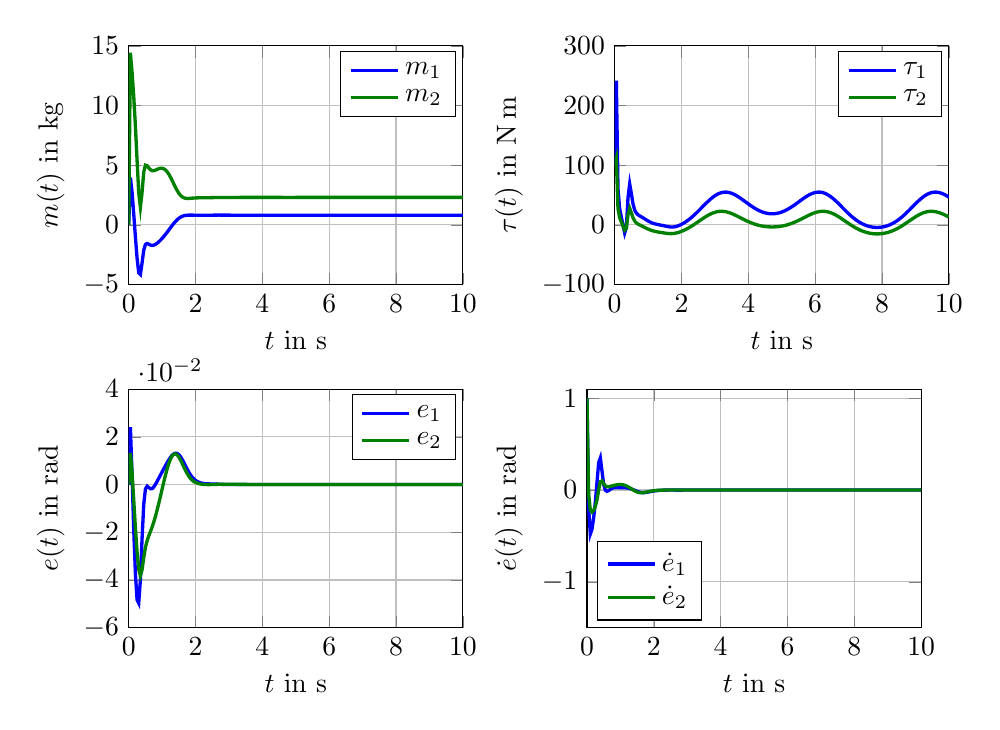
\begin{tikzpicture}

\begin{axis}[%
width=0.35\textwidth,
height=0.25\textwidth,
scale only axis,
xmin=0,
xmax=10,
xlabel={$t$ in $\mathrm{s}$},
xmajorgrids,
ymin=-1.5,
ymax=1.1,
ylabel={$\dot{e}(t)$ in $\mathrm{rad}$},
ymajorgrids,
name=plot1,
legend style={at={(0.03,0.03)},anchor=south west,draw=black,fill=white,legend cell align=left}
]
\addplot [
color=blue,
solid,
line width=1.2pt
]
table[row sep=crcr]{
0 1\\
0.05 -0.194509308945034\\
0.1 -0.479380867507292\\
0.15 -0.425880031881159\\
0.2 -0.301582691460445\\
0.25 -0.13260678308957\\
0.3 0.0834841574464273\\
0.35 0.299478265075243\\
0.4 0.350681459064839\\
0.45 0.204673782501047\\
0.5 0.0621156693705859\\
0.55 -0.00188652901090614\\
0.6 -0.0141822896033184\\
0.65 -0.0052483199426292\\
0.7 0.00790770656798701\\
0.75 0.0181719288096097\\
0.8 0.024007741070591\\
0.85 0.026383248044767\\
0.9 0.0268527083307829\\
0.95 0.0266250339483141\\
1 0.0263148584695381\\
1.05 0.0260315290711548\\
1.1 0.0255642315371086\\
1.15 0.0245516014595434\\
1.2 0.0226086313248532\\
1.25 0.0194190686580914\\
1.3 0.0148079699088137\\
1.35 0.00880247845940141\\
1.4 0.00167673211447736\\
1.45 -0.00603671232869479\\
1.5 -0.0135946307201054\\
1.55 -0.0201673205396507\\
1.6 -0.0250240458377644\\
1.65 -0.0277199654971781\\
1.7 -0.0282032170575825\\
1.75 -0.0267919398280836\\
1.8 -0.0240396986416258\\
1.85 -0.0205610507107731\\
1.9 -0.0168904902222489\\
1.95 -0.0134101355319293\\
2 -0.0103410302729022\\
2.05 -0.00777277877418897\\
2.1 -0.00570612455410696\\
2.15 -0.00409223766736322\\
2.2 -0.00286195995796901\\
2.25 -0.00194440863826162\\
2.3 -0.00127707459146242\\
2.35 -0.000810043647256009\\
2.4 -0.000506369202756707\\
2.45 -0.000339720227795604\\
2.5 -0.000289735439743977\\
2.55 -0.000335448059608723\\
2.6 -0.000448032246709085\\
2.65 -0.000585883644460106\\
2.7 -0.000696627828897345\\
2.75 -0.000729798413253158\\
2.8 -0.000658410788590302\\
2.85 -0.000498388820753592\\
2.9 -0.000308672662651777\\
2.95 -0.000162099968795792\\
3 -0.000100107302567931\\
3.05 -0.000105803207801403\\
3.1 -0.000122490717027635\\
3.15 -0.000104482749799795\\
3.2 -5.28229328414787e-05\\
3.25 -2.99675882020622e-06\\
3.3 1.70021353329552e-05\\
3.35 1.13667494501257e-05\\
3.4 3.34591240835902e-06\\
3.45 7.7021098580099e-06\\
3.5 2.04925390301369e-05\\
3.55 3.01448314372621e-05\\
3.6 3.11734935926067e-05\\
3.65 2.66703648508226e-05\\
3.7 2.2210111908616e-05\\
3.75 2.04491885350544e-05\\
3.8 2.06105278637292e-05\\
3.85 2.07987113668429e-05\\
3.9 1.98975335394813e-05\\
3.95 1.79103776248857e-05\\
4 1.53889584635358e-05\\
4.05 1.28489457147385e-05\\
4.1 1.05397636485094e-05\\
4.15 8.49056613605459e-06\\
4.2 6.64073702527634e-06\\
4.25 4.93715335475597e-06\\
4.3 3.37229132746364e-06\\
4.35 1.98210628671314e-06\\
4.4 8.2810487733731e-07\\
4.45 -2.15375733914058e-08\\
4.5 -5.06408881884024e-07\\
4.55 -5.83442753776531e-07\\
4.6 -2.32761035015572e-07\\
4.65 5.391878655156e-07\\
4.7 1.69854323967336e-06\\
4.75 3.18456614063073e-06\\
4.8 4.91139418794251e-06\\
4.85 6.77061721107708e-06\\
4.9 8.63438670972716e-06\\
4.95 1.03590742735471e-05\\
5 1.17899684558553e-05\\
5.05 1.27680348183112e-05\\
5.1 1.31401546516474e-05\\
5.15 1.27742116016183e-05\\
5.2 1.15795661308482e-05\\
5.25 9.53155321792298e-06\\
5.3 6.69564593092087e-06\\
5.35 3.24345148894345e-06\\
5.4 -5.4971302254625e-07\\
5.45 -4.3348590293979e-06\\
5.5 -7.74924361224283e-06\\
5.55 -1.04953056900836e-05\\
5.6 -1.24126557640158e-05\\
5.65 -1.3509518615229e-05\\
5.7 -1.39305139543744e-05\\
5.75 -1.38687397011061e-05\\
5.8 -1.34671872177305e-05\\
5.85 -1.27689927633678e-05\\
5.9 -1.17470459348734e-05\\
5.95 -1.03845630590182e-05\\
6 -8.73763712760933e-06\\
6.05 -6.92979132577154e-06\\
6.1 -5.09289659700318e-06\\
6.15 -3.31464031466666e-06\\
6.2 -1.63487852899991e-06\\
6.25 -7.76217951026226e-08\\
6.3 1.32404238006867e-06\\
6.35 2.53178942355436e-06\\
6.4 3.52055888597214e-06\\
6.45 4.28827538379029e-06\\
6.5 4.85026521146459e-06\\
6.55 5.22793742052663e-06\\
6.6 5.44162267235304e-06\\
6.65 5.50916338981633e-06\\
6.7 5.44660888401882e-06\\
6.75 5.26798722899624e-06\\
6.8 4.98380631597239e-06\\
6.85 4.5994176216535e-06\\
6.9 4.11435148639505e-06\\
6.95 3.5232356082604e-06\\
7 2.81860914619347e-06\\
7.05 1.99582405546739e-06\\
7.1 1.05996750532356e-06\\
7.15 3.40982025948122e-08\\
7.2 -1.03293965669771e-06\\
7.25 -2.06197001328956e-06\\
7.3 -2.94563115321722e-06\\
7.35 -3.55996276346637e-06\\
7.4 -3.78580651844151e-06\\
7.45 -3.53664533297993e-06\\
7.5 -2.78570749662199e-06\\
7.55 -1.58324844590219e-06\\
7.6 -5.64607146036344e-08\\
7.65 1.6104500783487e-06\\
7.7 3.21164221425696e-06\\
7.75 4.56045649925574e-06\\
7.8 5.52383243993676e-06\\
7.85 6.04120807713021e-06\\
7.9 6.12465147178942e-06\\
7.95 5.84322872841658e-06\\
8 5.29874096158456e-06\\
8.05 4.6008207370829e-06\\
8.1 3.84744354806066e-06\\
8.15 3.11364906896427e-06\\
8.2 2.44821570938303e-06\\
8.25 1.87613018293176e-06\\
8.3 1.40412114396637e-06\\
8.35 1.02692612624633e-06\\
8.4 7.32800439551262e-07\\
8.45 5.07615904865588e-07\\
8.5 3.37502440106441e-07\\
8.55 2.10306998926768e-07\\
8.6 1.16237859337787e-07\\
8.65 4.8014292652887e-08\\
8.7 7.25163262771389e-10\\
8.75 -2.85354810891647e-08\\
8.8 -4.13012012367986e-08\\
8.85 -3.87174692306758e-08\\
8.9 -2.28490966147632e-08\\
8.95 2.02567052021152e-09\\
9 2.88819572702437e-08\\
9.05 4.90869010993933e-08\\
9.1 5.55212832376029e-08\\
9.15 4.64672674782562e-08\\
9.2 2.74834707214566e-08\\
9.25 8.76327499454987e-09\\
9.3 -1.34823918696014e-09\\
9.35 -1.96273031161098e-09\\
9.4 7.3584394133519e-10\\
9.45 -1.77802883527534e-10\\
9.5 -6.19437767745978e-09\\
9.55 -1.32720836543143e-08\\
9.6 -1.69987226517065e-08\\
9.65 -1.68419628243655e-08\\
9.7 -1.5477539805353e-08\\
9.75 -1.52670330821891e-08\\
9.8 -1.62668452041714e-08\\
9.85 -1.71422146477695e-08\\
9.9 -1.69820549844601e-08\\
9.95 -1.59582248526746e-08\\
10 -1.47521415083673e-08\\
};
\addlegendentry{$\dot{e}_1$};

\addplot [
color=green!50!black,
solid,
line width=1.2pt
]
table[row sep=crcr]{
0 1\\
0.05 -0.042338993253243\\
0.1 -0.219449304897615\\
0.15 -0.240649948595194\\
0.2 -0.221661705616473\\
0.25 -0.178717114266024\\
0.3 -0.106497488136391\\
0.35 -7.05521343713489e-05\\
0.4 0.0908032132209942\\
0.45 0.0994235398778247\\
0.5 0.068863909750375\\
0.55 0.0461130314616438\\
0.6 0.0368806054434633\\
0.65 0.0362344264609977\\
0.7 0.0398590712802178\\
0.75 0.0450555739465863\\
0.8 0.0502880136549968\\
0.85 0.0547622850163882\\
0.9 0.0580848761339557\\
0.95 0.0600103175090783\\
1 0.060308842607822\\
1.05 0.0587432787078248\\
1.1 0.0551112590451396\\
1.15 0.0493095340439663\\
1.2 0.0413937906443125\\
1.25 0.0316222712575556\\
1.3 0.0204780992739629\\
1.35 0.00866417513848192\\
1.4 -0.00294024749026431\\
1.45 -0.0133741026807847\\
1.5 -0.0217434904462563\\
1.55 -0.0274022179460302\\
1.6 -0.0301067393371687\\
1.65 -0.0300736083597539\\
1.7 -0.0278997110432078\\
1.75 -0.0243749352956464\\
1.8 -0.0202720701951588\\
1.85 -0.0161964928906742\\
1.9 -0.0125292050997365\\
1.95 -0.00944628178151197\\
2 -0.00697613430054145\\
2.05 -0.00506129664511046\\
2.1 -0.00360707626898937\\
2.15 -0.00251274747714436\\
2.2 -0.00168809165182637\\
2.25 -0.00106020519778383\\
2.3 -0.000574962929690059\\
2.35 -0.000196072887079235\\
2.4 9.68515956014659e-05\\
2.45 0.000311027227812621\\
2.5 0.000444691146569642\\
2.55 0.000493510481016202\\
2.6 0.000459004499225868\\
2.65 0.000356653367210247\\
2.7 0.000219083188584102\\
2.75 8.95910581997228e-05\\
2.8 5.65362904714206e-06\\
2.85 -1.97832945416643e-05\\
2.9 -5.56125486983472e-06\\
2.95 1.09832037988866e-05\\
3 1.04805605238845e-06\\
3.05 -3.60080313313027e-05\\
3.1 -7.73263041586869e-05\\
3.15 -9.99757042378091e-05\\
3.2 -0.000100002360651885\\
3.25 -9.07528497686716e-05\\
3.3 -8.66299534684201e-05\\
3.35 -9.07959962325178e-05\\
3.4 -9.66665929493793e-05\\
3.45 -9.72986335906478e-05\\
3.5 -9.16324969210125e-05\\
3.55 -8.33997157063671e-05\\
3.6 -7.65077549241822e-05\\
3.65 -7.21424002435578e-05\\
3.7 -6.91730286582759e-05\\
3.75 -6.60789150807028e-05\\
3.8 -6.22445767022306e-05\\
3.85 -5.79873189175961e-05\\
3.9 -5.39324478842085e-05\\
3.95 -5.04954216893339e-05\\
4 -4.77489049943713e-05\\
4.05 -4.55466538282767e-05\\
4.1 -4.36891124611094e-05\\
4.15 -4.20171751633891e-05\\
4.2 -4.04294603514321e-05\\
4.25 -3.88623930891452e-05\\
4.3 -3.72668484902583e-05\\
4.35 -3.55953821805644e-05\\
4.4 -3.38000912355474e-05\\
4.45 -3.18361854039773e-05\\
4.5 -2.9666731567457e-05\\
4.55 -2.72659997325175e-05\\
4.6 -2.46205276463324e-05\\
4.65 -2.17280217536253e-05\\
4.7 -1.85947001584662e-05\\
4.75 -1.52319027486025e-05\\
4.8 -1.16528888151196e-05\\
4.85 -7.87075925967606e-06\\
4.9 -3.89836910891228e-06\\
4.95 2.49098804055992e-07\\
5 4.54859469806168e-06\\
5.05 8.96098560776437e-06\\
5.1 1.34213082628731e-05\\
5.15 1.78297305938324e-05\\
5.2 2.20466010844023e-05\\
5.25 2.58956986060044e-05\\
5.3 2.91793691596931e-05\\
5.35 3.17067699574514e-05\\
5.4 3.33314722629208e-05\\
5.45 3.39880650774838e-05\\
5.5 3.37121686270203e-05\\
5.55 3.2629261041528e-05\\
5.6 3.09089541036256e-05\\
5.65 2.87011305764029e-05\\
5.7 2.60876812838706e-05\\
5.75 2.30819811724015e-05\\
5.8 1.96797992951803e-05\\
5.85 1.59255901651667e-05\\
5.9 1.19418678523608e-05\\
5.95 7.89887815233481e-06\\
6 3.95481548587373e-06\\
6.05 2.20139736994973e-07\\
6.1 -3.23214654074366e-06\\
6.15 -6.33768867619455e-06\\
6.2 -9.03160195953046e-06\\
6.25 -1.12645238595777e-05\\
6.3 -1.30200547977521e-05\\
6.35 -1.43150999301067e-05\\
6.4 -1.51874964317011e-05\\
6.45 -1.56848561607692e-05\\
6.5 -1.58605713810323e-05\\
6.55 -1.57735164236783e-05\\
6.6 -1.5486882629423e-05\\
6.65 -1.50652763832859e-05\\
6.7 -1.45715694002124e-05\\
6.75 -1.4064662148372e-05\\
6.8 -1.35980952158388e-05\\
6.85 -1.32187248591542e-05\\
6.9 -1.29646013238283e-05\\
6.95 -1.28614172483221e-05\\
7 -1.29172685149337e-05\\
7.05 -1.31160572913736e-05\\
7.1 -1.3410751869336e-05\\
7.15 -1.37188084611273e-05\\
7.2 -1.39229746666247e-05\\
7.25 -1.3880786749132e-05\\
7.3 -1.34446675983391e-05\\
7.35 -1.24913723437703e-05\\
7.4 -1.09552507592259e-05\\
7.45 -8.85606267853056e-06\\
7.5 -6.31104307124986e-06\\
7.55 -3.52404325082434e-06\\
7.6 -7.51505724538859e-07\\
7.65 1.74675565361992e-06\\
7.7 3.75814003722441e-06\\
7.75 5.15470367007387e-06\\
7.8 5.9078500231069e-06\\
7.85 6.07880461726915e-06\\
7.9 5.79115732669833e-06\\
7.95 5.19604678343721e-06\\
8 4.44037921812357e-06\\
8.05 3.64491104098974e-06\\
8.1 2.89428638144962e-06\\
8.15 2.23723884584803e-06\\
8.2 1.69317917775302e-06\\
8.25 1.26125496408003e-06\\
8.3 9.28989693338433e-07\\
8.35 6.78976412538113e-07\\
8.4 4.93248726418649e-07\\
8.45 3.55650339733948e-07\\
8.5 2.52800541833409e-07\\
8.55 1.7424946041622e-07\\
8.6 1.12280098885087e-07\\
8.65 6.16420881005553e-08\\
8.7 1.93364330103307e-08\\
8.75 -1.55800820023089e-08\\
8.8 -4.23296775409199e-08\\
8.85 -5.91082692791289e-08\\
8.9 -6.42721921240152e-08\\
8.95 -5.78343938295589e-08\\
9 -4.26164170619359e-08\\
9.05 -2.4114905072814e-08\\
9.1 -8.54328241484126e-09\\
9.15 2.389816122772e-10\\
9.2 2.86873624855133e-09\\
9.25 3.7204159752946e-09\\
9.3 7.39730199317279e-09\\
9.35 1.52201996561629e-08\\
9.4 2.47252655016794e-08\\
9.45 3.23721991435377e-08\\
9.5 3.66115825434221e-08\\
9.55 3.8504259891603e-08\\
9.6 3.99404064266307e-08\\
9.65 4.17435380706266e-08\\
9.7 4.3389903114921e-08\\
9.75 4.40291604286713e-08\\
9.8 4.34268581095409e-08\\
9.85 4.2036458314243e-08\\
9.9 4.04766530293088e-08\\
9.95 3.90806951244826e-08\\
10 3.78413637092123e-08\\
};
\addlegendentry{$\dot{e}_2$};

\end{axis}

\begin{axis}[%
width=0.35\textwidth,
height=0.25\textwidth,
scale only axis,
xmin=0,
xmax=10,
xlabel={$t$ in $\mathrm{s}$},
xmajorgrids,
ymin=-0.06,
ymax=0.04,
ylabel={$e(t)$ in $\mathrm{rad}$},
ymajorgrids,
name=plot3,
at=(plot1.left of south west),
anchor=right of south east,
legend style={draw=black,fill=white,legend cell align=left}
]
\addplot [
color=blue,
solid,
line width=1.2pt
]
table[row sep=crcr]{
0 0\\
0.05 0.0240614172663856\\
0.1 0.00425648693795412\\
0.15 -0.0188612856550443\\
0.2 -0.037236564742274\\
0.25 -0.0482868462614925\\
0.3 -0.0496898636071577\\
0.35 -0.0398479970980442\\
0.4 -0.0225572372090287\\
0.45 -0.00826370526426129\\
0.5 -0.0019051597696596\\
0.55 -0.000692441279682932\\
0.6 -0.00123573310530123\\
0.65 -0.00176505893980372\\
0.7 -0.00169563413680607\\
0.75 -0.00102549800866403\\
0.8 4.64354503166842e-05\\
0.85 0.00131734508023551\\
0.9 0.002653229231522\\
0.95 0.00399134728863437\\
1 0.00531464243002422\\
1.05 0.0066234558364312\\
1.1 0.00791480903038866\\
1.15 0.00917080030898088\\
1.2 0.0103544234945629\\
1.25 0.0114108071882204\\
1.3 0.0122725243801545\\
1.35 0.0128682244371511\\
1.4 0.01313395323024\\
1.45 0.0130259796999835\\
1.5 0.0125328209310294\\
1.55 0.0116829911485781\\
1.6 0.0105448521948341\\
1.65 0.00921682719482086\\
1.7 0.00780994648173239\\
1.75 0.00642821387082892\\
1.8 0.00515313261297934\\
1.85 0.00403630081190154\\
1.9 0.00310013652903018\\
1.95 0.00234398919094336\\
2 0.00175219453953746\\
2.05 0.00130148903439653\\
2.1 0.000966529365082791\\
2.15 0.000723319356340291\\
2.2 0.000550911174601931\\
2.25 0.000431915734148025\\
2.3 0.000352306703351402\\
2.35 0.000300876698169472\\
2.4 0.000268585204039384\\
2.45 0.000247958895434719\\
2.5 0.000232667928041996\\
2.55 0.000217385319926766\\
2.6 0.000198000469327275\\
2.65 0.000172153679985743\\
2.7 0.000139863732262491\\
2.75 0.000103796406869916\\
2.8 6.86512754745072e-05\\
2.85 3.9458305351181e-05\\
2.9 1.93161079896087e-05\\
2.95 7.85312276097017e-06\\
3 1.66054511746561e-06\\
3.05 -3.3102823444181e-06\\
3.1 -9.09533580046445e-06\\
3.15 -1.49507607292172e-05\\
3.2 -1.89605589498085e-05\\
3.25 -2.02683761039296e-05\\
3.3 -1.97772710493205e-05\\
3.35 -1.90058665626158e-05\\
3.4 -1.86728804544289e-05\\
3.45 -1.84516379193034e-05\\
3.5 -1.77564792926965e-05\\
3.55 -1.6457730434849e-05\\
3.6 -1.4889846867705e-05\\
3.65 -1.34325909624256e-05\\
3.7 -1.22188739011264e-05\\
3.75 -1.11633322293914e-05\\
3.8 -1.01402421912589e-05\\
3.85 -9.10132511644512e-06\\
3.9 -8.07819509351937e-06\\
3.95 -7.12900159083318e-06\\
4 -6.29509008731599e-06\\
4.05 -5.58936803163324e-06\\
4.1 -5.00538122449878e-06\\
4.15 -4.53020975799134e-06\\
4.2 -4.15224371597134e-06\\
4.25 -3.86299317700622e-06\\
4.3 -3.65553864301038e-06\\
4.35 -3.52219234833751e-06\\
4.4 -3.45274620805469e-06\\
4.45 -3.43367919497517e-06\\
4.5 -3.44820624187392e-06\\
4.55 -3.47692414182088e-06\\
4.6 -3.49883802053252e-06\\
4.65 -3.49260885845748e-06\\
4.7 -3.43790453860571e-06\\
4.75 -3.31676304354822e-06\\
4.8 -3.11489673165966e-06\\
4.85 -2.82288678910003e-06\\
4.9 -2.43723483772662e-06\\
4.95 -1.96124629192607e-06\\
5 -1.40570800521989e-06\\
5.05 -7.8928479219087e-07\\
5.1 -1.38497241120028e-07\\
5.15 5.12928891582831e-07\\
5.2 1.12560314058374e-06\\
5.25 1.65714627986535e-06\\
5.3 2.06610825448372e-06\\
5.35 2.31692940211303e-06\\
5.4 2.38528517360059e-06\\
5.45 2.26264828873113e-06\\
5.5 1.95858809581839e-06\\
5.55 1.49952047845403e-06\\
5.6 9.23550320552913e-07\\
5.65 2.72593002725863e-07\\
5.7 -4.15529507913348e-07\\
5.75 -1.11187355678055e-06\\
5.8 -1.79624954926849e-06\\
5.85 -2.45316686575681e-06\\
5.9 -3.06726289872605e-06\\
5.95 -3.6217250220516e-06\\
6 -4.10058945482517e-06\\
6.05 -4.4925555871822e-06\\
6.1 -4.79299049149784e-06\\
6.15 -5.00287843049896e-06\\
6.2 -5.12630094468003e-06\\
6.25 -5.16878232353912e-06\\
6.3 -5.13722395661248e-06\\
6.35 -5.04037322310302e-06\\
6.4 -4.88862918118782e-06\\
6.45 -4.69307077199943e-06\\
6.5 -4.46439891915729e-06\\
6.55 -4.21235342240589e-06\\
6.6 -3.94561642913516e-06\\
6.65 -3.67192016298423e-06\\
6.7 -3.39815459160508e-06\\
6.75 -3.13045615257801e-06\\
6.8 -2.87434252310703e-06\\
6.85 -2.63493117480529e-06\\
6.9 -2.41721905147596e-06\\
6.95 -2.22635766766732e-06\\
7 -2.06783599820959e-06\\
7.05 -1.94747104032e-06\\
7.1 -1.87110157012782e-06\\
7.15 -1.84389811963559e-06\\
7.2 -1.86926204692739e-06\\
7.25 -1.94740187753339e-06\\
7.3 -2.0738355813732e-06\\
7.35 -2.23822836320497e-06\\
7.4 -2.4240607117143e-06\\
7.45 -2.60955009101504e-06\\
7.5 -2.76998228720959e-06\\
7.55 -2.88119004487886e-06\\
7.6 -2.92348466035541e-06\\
7.65 -2.88508351398153e-06\\
7.7 -2.76412297872675e-06\\
7.75 -2.5687173519362e-06\\
7.8 -2.31508999615215e-06\\
7.85 -2.0243443826784e-06\\
7.9 -1.7187596531576e-06\\
7.95 -1.41849714407893e-06\\
8 -1.13933833678637e-06\\
8.05 -8.91682891301926e-07\\
8.1 -6.80675287578758e-07\\
8.15 -5.07105292646415e-07\\
8.2 -3.68667439132331e-07\\
8.25 -2.6123078555873e-07\\
8.3 -1.79897499341664e-07\\
8.35 -1.1975833058564e-07\\
8.4 -7.6349341071591e-08\\
8.45 -4.58672003711413e-08\\
8.5 -2.52166552083821e-08\\
8.55 -1.19569463219449e-08\\
8.6 -4.19715229238449e-09\\
8.65 -4.72794803307863e-10\\
8.7 3.77228803749574e-10\\
8.75 -6.78936795672769e-10\\
8.8 -2.78023892796853e-09\\
8.85 -5.12697639898363e-09\\
8.9 -6.9929537716007e-09\\
8.95 -7.80489173290988e-09\\
9 -7.27136234557335e-09\\
9.05 -5.49992007492506e-09\\
9.1 -3.00649027895616e-09\\
9.15 -5.40800182413648e-10\\
9.2 1.24512564148027e-09\\
9.25 2.11470138622438e-09\\
9.3 2.32371945296794e-09\\
9.35 2.36972629019672e-09\\
9.4 2.5966406837219e-09\\
9.45 2.98297238646161e-09\\
9.5 3.27525481735869e-09\\
9.55 3.29284320643719e-09\\
9.6 3.087764210985e-09\\
9.65 2.84248033444179e-09\\
9.7 2.67426514266589e-09\\
9.75 2.56222104644266e-09\\
9.8 2.42608622080809e-09\\
9.85 2.22816415318405e-09\\
9.9 1.99546235091219e-09\\
9.95 1.77509984489177e-09\\
10 1.59094426521733e-09\\
};
\addlegendentry{$e_1$};

\addplot [
color=green!50!black,
solid,
line width=1.2pt
]
table[row sep=crcr]{
0 0\\
0.05 0.0131941833924348\\
0.1 0.00537906188274924\\
0.15 -0.00638613654795661\\
0.2 -0.0180524485560637\\
0.25 -0.028162861823795\\
0.3 -0.0354397453102917\\
0.35 -0.0382095865778552\\
0.4 -0.0356744768912289\\
0.45 -0.0305991982564586\\
0.5 -0.0263696734241109\\
0.55 -0.0235571552357503\\
0.6 -0.0215292694560409\\
0.65 -0.0197268188103842\\
0.7 -0.0178355780617864\\
0.75 -0.0157153482099367\\
0.8 -0.013329826880404\\
0.85 -0.0106993971424307\\
0.9 -0.00787286411592691\\
0.95 -0.00491419402814364\\
1 -0.00189893692778198\\
1.05 0.00108560618915354\\
1.1 0.00394089653675611\\
1.15 0.00656048282444577\\
1.2 0.00883650419294346\\
1.25 0.0106688073276943\\
1.3 0.0119757308425942\\
1.35 0.0127053549082564\\
1.4 0.0128455923331869\\
1.45 0.0124308760659326\\
1.5 0.0115427306049024\\
1.55 0.0103019368646511\\
1.6 0.00885201281115566\\
1.65 0.00733711128875492\\
1.7 0.00588044184841452\\
1.75 0.00456964251358349\\
1.8 0.0034524851024349\\
1.85 0.00254185246204763\\
1.9 0.00182591637667662\\
1.95 0.00127911201298259\\
2 0.000871030169106835\\
2.05 0.000572225547895822\\
2.1 0.000357222759473363\\
2.15 0.00020552776638838\\
2.2 0.000101464976572707\\
2.25 3.34512362278883e-05\\
2.3 -6.92144859537613e-06\\
2.35 -2.58071875877119e-05\\
2.4 -2.79525771290645e-05\\
2.45 -1.74278776580161e-05\\
2.5 1.81132443022314e-06\\
2.55 2.56253341799351e-05\\
2.6 4.97669095460562e-05\\
2.65 7.03861250140325e-05\\
2.7 8.48397959137825e-05\\
2.75 9.24331974801462e-05\\
2.8 9.45735429704886e-05\\
2.85 9.39935600706154e-05\\
2.9 9.3268116712425e-05\\
2.95 9.3471135504869e-05\\
3 9.39075075572782e-05\\
3.05 9.31089467104268e-05\\
3.1 9.02351320121522e-05\\
3.15 8.56983582896882e-05\\
3.2 8.06235993281584e-05\\
3.25 7.58508090869386e-05\\
3.3 7.14530635518573e-05\\
3.35 6.70409601655764e-05\\
3.4 6.23422501949134e-05\\
3.45 5.74624277331903e-05\\
3.5 5.27171641394042e-05\\
3.55 4.8338779658097e-05\\
3.6 4.43499873484243e-05\\
3.65 4.06414654688936e-05\\
3.7 3.7109350649156e-05\\
3.75 3.37239430346914e-05\\
3.8 3.05115398135936e-05\\
3.85 2.75039573998104e-05\\
3.9 2.47066370465676e-05\\
3.95 2.20976369095238e-05\\
4 1.96429708088086e-05\\
4.05 1.73112330463798e-05\\
4.1 1.50802394882632e-05\\
4.15 1.29369798550494e-05\\
4.2 1.08749179272838e-05\\
4.25 8.89153312033653e-06\\
4.3 6.98704337565026e-06\\
4.35 5.16405298112144e-06\\
4.4 3.42755709481501e-06\\
4.45 1.78488838098456e-06\\
4.5 2.45440754609305e-07\\
4.55 -1.17981582081761e-06\\
4.6 -2.47893189653237e-06\\
4.65 -3.63957244708946e-06\\
4.7 -4.64951376455414e-06\\
4.75 -5.49698548257815e-06\\
4.8 -6.17084385823308e-06\\
4.85 -6.66060921938882e-06\\
4.9 -6.95644596548917e-06\\
4.95 -7.04920253458141e-06\\
5 -6.93065396695225e-06\\
5.05 -6.59409112790943e-06\\
5.1 -6.03536592214127e-06\\
5.15 -5.25441793974846e-06\\
5.2 -4.25716698371215e-06\\
5.25 -3.05746558892928e-06\\
5.3 -1.67860395117181e-06\\
5.35 -1.53726926521713e-07\\
5.4 1.47542406558898e-06\\
5.45 3.16168112157733e-06\\
5.5 4.85710503261849e-06\\
5.55 6.5179074285604e-06\\
5.6 8.10792719896369e-06\\
5.65 9.59925472199252e-06\\
5.7 1.09698954909865e-05\\
5.75 1.22001205179467e-05\\
5.8 1.32701471913799e-05\\
5.85 1.41609660718744e-05\\
5.9 1.4857750314623e-05\\
5.95 1.53532241771726e-05\\
6 1.56485618587054e-05\\
6.05 1.57517050401734e-05\\
6.1 1.56750676031381e-05\\
6.15 1.54343959907488e-05\\
6.2 1.50486885325263e-05\\
6.25 1.45398823852144e-05\\
6.3 1.39315891327513e-05\\
6.35 1.32473591305526e-05\\
6.4 1.25093043469859e-05\\
6.45 1.17373610767357e-05\\
6.5 1.09489324908174e-05\\
6.55 1.01586150978439e-05\\
6.6 9.37794854810603e-06\\
6.65 8.61526929335499e-06\\
6.7 7.87572128990721e-06\\
6.75 7.16140268963716e-06\\
6.8 6.47160037359207e-06\\
6.85 5.80308841391375e-06\\
6.9 5.15050952176743e-06\\
6.95 4.50689652020664e-06\\
7 3.86441368493973e-06\\
7.05 3.21539713699082e-06\\
7.1 2.5537360551775e-06\\
7.15 1.87654880356991e-06\\
7.2 1.18596802389792e-06\\
7.25 4.90680478582028e-07\\
7.3 -1.93270316528604e-07\\
7.35 -8.42933792766232e-07\\
7.4 -1.43050177248139e-06\\
7.45 -1.92692843792308e-06\\
7.5 -2.30658712763177e-06\\
7.55 -2.55197497223136e-06\\
7.6 -2.65727895754075e-06\\
7.65 -2.62981227161507e-06\\
7.7 -2.48889193732449e-06\\
7.75 -2.26246175605294e-06\\
7.8 -1.98238766957459e-06\\
7.85 -1.67963577213381e-06\\
7.9 -1.38041341035677e-06\\
7.95 -1.10391408336685e-06\\
8 -8.61764944737331e-07\\
8.05 -6.58835363709365e-07\\
8.1 -4.94841869369544e-07\\
8.15 -3.66183937283715e-07\\
8.2 -2.67592805802686e-07\\
8.25 -1.93374386947553e-07\\
8.3 -1.38200506261121e-07\\
8.35 -9.75131827507525e-08\\
8.4 -6.7652544899488e-08\\
8.45 -4.58184284957142e-08\\
8.5 -2.99512568080473e-08\\
8.55 -1.85871531499515e-08\\
8.6 -1.07157006601355e-08\\
8.65 -5.65017377329724e-09\\
8.7 -2.90999879748455e-09\\
8.75 -2.11313033737781e-09\\
8.8 -2.88087020905436e-09\\
8.85 -4.76759365319879e-09\\
8.9 -7.23752047182558e-09\\
8.95 -9.71030594820732e-09\\
9 -1.16765313529221e-08\\
9.05 -1.28423928158483e-08\\
9.1 -1.32220537296668e-08\\
9.15 -1.30976801071547e-08\\
9.2 -1.28384670117221e-08\\
9.25 -1.26789841681241e-08\\
9.3 -1.26099362757204e-08\\
9.35 -1.2458255913006e-08\\
9.4 -1.20759176443219e-08\\
9.45 -1.14676471443809e-08\\
9.5 -1.07614960970226e-08\\
9.55 -1.00829243704359e-08\\
9.6 -9.46660105860531e-09\\
9.65 -8.87148976502772e-09\\
9.7 -8.25293855477582e-09\\
9.75 -7.61010621186387e-09\\
9.8 -6.97733970600467e-09\\
9.85 -6.38808766995069e-09\\
9.9 -5.85199855240859e-09\\
9.95 -5.35837552106955e-09\\
10 -4.89244811330281e-09\\
};
\addlegendentry{$e_2$};

\end{axis}

\begin{axis}[%
width=0.35\textwidth,
height=0.25\textwidth,
scale only axis,
xmin=0,
xmax=10,
xlabel={$t$ in $\mathrm{s}$},
xmajorgrids,
ymin=-5,
ymax=15,
ylabel={$m(t)$ in $\mathrm{kg}$},
ymajorgrids,
name=plot2,
at=(plot3.above north west),
anchor=below south west,
legend style={draw=black,fill=white,legend cell align=left}
]
\addplot [
color=blue,
solid,
line width=1.2pt
]
table[row sep=crcr]{
0 0\\
0.05 3.96515377468506\\
0.1 2.75102083024893\\
0.15 0.929117119760223\\
0.2 -1.00851181894507\\
0.25 -2.78817355594742\\
0.3 -4.01469517814325\\
0.35 -4.15958046723056\\
0.4 -3.17678841588952\\
0.45 -2.11969366730519\\
0.5 -1.64609267782358\\
0.55 -1.56633238139465\\
0.6 -1.62629056380487\\
0.65 -1.69518955346721\\
0.7 -1.72292588780113\\
0.75 -1.70029113940821\\
0.8 -1.63520777418819\\
0.85 -1.53920800221634\\
0.9 -1.42132695443925\\
0.95 -1.2868431500492\\
1 -1.13829027162119\\
1.05 -0.976973875972881\\
1.1 -0.804201296302356\\
1.15 -0.622045502654055\\
1.2 -0.433700552114799\\
1.25 -0.243520893410031\\
1.3 -0.056806823458486\\
1.35 0.120628118290889\\
1.4 0.283068833920952\\
1.45 0.425612840644229\\
1.5 0.544853053598216\\
1.55 0.639355232521155\\
1.6 0.709779056547017\\
1.65 0.758594845131718\\
1.7 0.789488667780023\\
1.75 0.806647270118553\\
1.8 0.814120209852964\\
1.85 0.815385155831986\\
1.9 0.813147395130895\\
1.95 0.80933218940526\\
2 0.805196439451715\\
2.05 0.801488485142955\\
2.1 0.798605657747847\\
2.15 0.796723118407224\\
2.2 0.795885788431421\\
2.25 0.796065578043281\\
2.3 0.797190234782817\\
2.35 0.799150742694428\\
2.4 0.80179388459911\\
2.45 0.804907221618835\\
2.5 0.808206279157959\\
2.55 0.811337528162491\\
2.6 0.81391271148559\\
2.65 0.815584440558943\\
2.7 0.816154080095581\\
2.75 0.815672145676609\\
2.8 0.814465517675967\\
2.85 0.81303566664931\\
2.9 0.811840140011607\\
2.95 0.811070681608498\\
3 0.810589019128435\\
3.05 0.810091221114207\\
3.1 0.809379789083879\\
3.15 0.808510369910905\\
3.2 0.807693666754302\\
3.25 0.807076182092444\\
3.3 0.806629192801412\\
3.35 0.806229148795058\\
3.4 0.805801987658472\\
3.45 0.805372500428733\\
3.5 0.805002755297153\\
3.55 0.804718644551869\\
3.6 0.804498086805057\\
3.65 0.804306170747201\\
3.7 0.804125705438449\\
3.75 0.803959482012049\\
3.8 0.803816217034811\\
3.85 0.803699342730615\\
3.9 0.803605369626404\\
3.95 0.803527737303925\\
4 0.803460548160432\\
4.05 0.803399951522968\\
4.1 0.803343767579607\\
4.15 0.803290624659822\\
4.2 0.803239362281728\\
4.25 0.803188837912257\\
4.3 0.803137987713852\\
4.35 0.803085968371539\\
4.4 0.803032279995776\\
4.45 0.802976837368987\\
4.5 0.802919991598219\\
4.55 0.802862514492933\\
4.6 0.80280555709832\\
4.65 0.802750590178232\\
4.7 0.802699331237037\\
4.75 0.802653660309337\\
4.8 0.802615524836499\\
4.85 0.802586832243065\\
4.9 0.802569327511184\\
4.95 0.802564452730501\\
5 0.802573187166593\\
5.05 0.802595870825626\\
5.1 0.802632022544593\\
5.15 0.802680175281036\\
5.2 0.802737764935447\\
5.25 0.802801120712548\\
5.3 0.802865607848326\\
5.35 0.802925958714509\\
5.4 0.802976788653093\\
5.45 0.803013229247754\\
5.5 0.803031540596057\\
5.55 0.803029520530571\\
5.6 0.803006555940103\\
5.65 0.802963282753968\\
5.7 0.80290100441562\\
5.75 0.80282116338474\\
5.8 0.802725144993799\\
5.85 0.802614478479188\\
5.9 0.802491209427551\\
5.95 0.802358083368016\\
6 0.802218341778338\\
6.05 0.80207526415052\\
6.1 0.80193178432546\\
6.15 0.801790387023031\\
6.2 0.801653204568186\\
6.25 0.801522092884573\\
6.3 0.801398578347896\\
6.35 0.801283752016958\\
6.4 0.801178234824406\\
6.45 0.801082243962885\\
6.5 0.800995699771781\\
6.55 0.800918309659019\\
6.6 0.800849614835761\\
6.65 0.800789018882681\\
6.7 0.800735815086779\\
6.75 0.800689214011248\\
6.8 0.800648364821194\\
6.85 0.800612366140165\\
6.9 0.800580267942447\\
6.95 0.800551070229016\\
7 0.800523726218526\\
7.05 0.800497158355736\\
7.1 0.800470294840391\\
7.15 0.800442131890659\\
7.2 0.800411821655502\\
7.25 0.800378777476623\\
7.3 0.800342778578201\\
7.35 0.800304048494073\\
7.4 0.800263279766713\\
7.45 0.800221584793377\\
7.5 0.800180369109459\\
7.55 0.800141144608033\\
7.6 0.800105318783993\\
7.65 0.800074004664212\\
7.7 0.800047890893511\\
7.75 0.800027194360557\\
7.8 0.800011695343839\\
7.85 0.800000835490717\\
7.9 0.799993847939537\\
7.95 0.799989888295293\\
8 0.799988142739353\\
8.05 0.799987900939022\\
8.1 0.79998859233383\\
8.15 0.799989792050306\\
8.2 0.799991206283927\\
8.25 0.799992647106653\\
8.3 0.799994004636787\\
8.35 0.799995221698217\\
8.4 0.799996273481788\\
8.45 0.799997152808393\\
8.5 0.799997860490715\\
8.55 0.799998399865745\\
8.6 0.799998774591727\\
8.65 0.799998989026718\\
8.7 0.799999050703692\\
8.75 0.799998974377724\\
8.8 0.799998786671524\\
8.85 0.799998529462571\\
8.9 0.799998259182934\\
8.95 0.799998039066262\\
9 0.799997923408575\\
9.05 0.799997937808991\\
9.1 0.799998065371088\\
9.15 0.799998250842885\\
9.2 0.799998426980724\\
9.25 0.799998550936676\\
9.3 0.799998625568832\\
9.35 0.799998687441009\\
9.4 0.799998770481237\\
9.45 0.799998877568504\\
9.5 0.799998984688095\\
9.55 0.799999068812373\\
9.6 0.799999128277099\\
9.65 0.799999177679525\\
9.7 0.79999922916725\\
9.75 0.79999928242818\\
9.8 0.799999330009648\\
9.85 0.799999367208087\\
9.9 0.799999395511052\\
9.95 0.799999419207189\\
10 0.799999441168637\\
};
\addlegendentry{$m_1$};

\addplot [
color=green!50!black,
solid,
line width=1.2pt
]
table[row sep=crcr]{
0 0\\
0.05 14.4147403160311\\
0.1 12.816856592172\\
0.15 10.786267151516\\
0.2 8.302294370554\\
0.25 5.41506975438675\\
0.3 2.68111065180416\\
0.35 1.4691532589113\\
0.4 2.72678419948933\\
0.45 4.41609282796532\\
0.5 4.99810748779216\\
0.55 4.95505248610045\\
0.6 4.76898565154931\\
0.65 4.61638105704737\\
0.7 4.54154342067607\\
0.75 4.53846022752724\\
0.8 4.58263271978028\\
0.85 4.64648378899582\\
0.9 4.70615952642872\\
0.95 4.74308094032056\\
1 4.74338938936299\\
1.05 4.69728293833459\\
1.1 4.59887591925963\\
1.15 4.44647362465364\\
1.2 4.24296572994491\\
1.25 3.99606915627984\\
1.3 3.71819128424049\\
1.35 3.42569398084899\\
1.4 3.13736663226165\\
1.45 2.87205293489144\\
1.5 2.64569304736578\\
1.55 2.46848633010861\\
1.6 2.34318266385314\\
1.65 2.26530181252466\\
1.7 2.22527244982767\\
1.75 2.21155237325754\\
1.8 2.21343954212957\\
1.85 2.22271883331593\\
1.9 2.23405279079928\\
1.95 2.24454400468343\\
2 2.25298978090139\\
2.05 2.25918266054888\\
2.1 2.2634032707091\\
2.15 2.26611476251158\\
2.2 2.26780968969339\\
2.25 2.26895067880451\\
2.3 2.26995663866238\\
2.35 2.2711999936728\\
2.4 2.27299181793467\\
2.45 2.27554189897863\\
2.5 2.2788940386414\\
2.55 2.28285705263625\\
2.6 2.28697638831605\\
2.65 2.29060510200183\\
2.7 2.29310985092532\\
2.75 2.29416874774469\\
2.8 2.29400790967901\\
2.85 2.29337199233097\\
2.9 2.29313930952444\\
2.95 2.29377192352052\\
3 2.2950202309962\\
3.05 2.29618055080412\\
3.1 2.29672063125117\\
3.15 2.2966993507126\\
3.2 2.29659653814912\\
3.25 2.29678578821983\\
3.3 2.29722527615937\\
3.35 2.29762420397621\\
3.4 2.29779751513983\\
3.45 2.29780368683523\\
3.5 2.29780399659336\\
3.55 2.29788056341396\\
3.6 2.29799999624137\\
3.65 2.29809344710712\\
3.7 2.2981295847877\\
3.75 2.29812200921931\\
3.8 2.29809817744629\\
3.85 2.29807429650659\\
3.9 2.29805155233928\\
3.95 2.29802431003447\\
4 2.29798788639536\\
4.05 2.29794126921834\\
4.1 2.29788625447608\\
4.15 2.29782570920651\\
4.2 2.29776241737377\\
4.25 2.29769868675722\\
4.3 2.29763637786434\\
4.35 2.29757703306478\\
4.4 2.29752195564473\\
4.45 2.29747221830438\\
4.5 2.29742863454166\\
4.55 2.29739173205726\\
4.6 2.29736175460957\\
4.65 2.29733870366759\\
4.7 2.29732241911183\\
4.75 2.29731268971213\\
4.8 2.29730937849074\\
4.85 2.29731254463112\\
4.9 2.2973225417504\\
4.95 2.29734007175694\\
5 2.29736617423585\\
5.05 2.29740213417331\\
5.1 2.29744929768858\\
5.15 2.29750879894516\\
5.2 2.29758122401575\\
5.25 2.29766626920859\\
5.3 2.29776248651808\\
5.35 2.29786723277972\\
5.4 2.29797692811942\\
5.45 2.2980876585089\\
5.5 2.29819601962557\\
5.55 2.29829993154068\\
5.6 2.29839905012097\\
5.65 2.29849448210704\\
5.7 2.2985878310582\\
5.75 2.29868003678533\\
5.8 2.29877070952717\\
5.85 2.29885840757375\\
5.9 2.29894162412447\\
5.95 2.29901966819268\\
6 2.2990927355754\\
6.05 2.29916124259204\\
6.1 2.29922517070643\\
6.15 2.29928403544698\\
6.2 2.29933735499159\\
6.25 2.29938502776503\\
6.3 2.29942728248584\\
6.35 2.29946438915762\\
6.4 2.29949648071308\\
6.45 2.2995235903894\\
6.5 2.29954576533667\\
6.55 2.29956311424111\\
6.6 2.29957577610355\\
6.65 2.29958387358651\\
6.7 2.29958749847691\\
6.75 2.2995867343773\\
6.8 2.29958170308887\\
6.85 2.2995726259826\\
6.9 2.29955990022581\\
6.95 2.29954419047417\\
7 2.29952652899856\\
7.05 2.29950840474226\\
7.1 2.29949180847995\\
7.15 2.29947919202116\\
7.2 2.2994733010347\\
7.25 2.29947686054055\\
7.3 2.29949213215869\\
7.35 2.29952041605417\\
7.4 2.29956161969571\\
7.45 2.29961403456488\\
7.5 2.29967443046352\\
7.55 2.29973849411623\\
7.6 2.29980152968061\\
7.65 2.29985924728465\\
7.7 2.29990843291687\\
7.75 2.29994733493885\\
7.8 2.29997570064185\\
7.85 2.29999450753852\\
7.9 2.30000551386192\\
7.95 2.30001077646544\\
8 2.30001225537121\\
8.05 2.30001156634334\\
8.1 2.30000988450444\\
8.15 2.30000796286951\\
8.2 2.30000621551571\\
8.25 2.30000482060347\\
8.3 2.30000381364256\\
8.35 2.30000315738338\\
8.4 2.3000027864763\\
8.45 2.30000263135404\\
8.5 2.30000262776681\\
8.55 2.30000271791514\\
8.6 2.30000284781314\\
8.65 2.30000296436075\\
8.7 2.30000301491411\\
8.75 2.30000295162884\\
8.8 2.3000027417404\\
8.85 2.30000238230606\\
8.9 2.30000191349655\\
8.95 2.30000142001151\\
9 2.30000101011219\\
9.05 2.30000077141306\\
9.1 2.300000721755\\
9.15 2.30000078976351\\
9.2 2.30000085200214\\
9.25 2.30000081343462\\
9.3 2.30000067232549\\
9.35 2.30000051069334\\
9.4 2.30000041484867\\
9.45 2.30000040082624\\
9.5 2.30000041518687\\
9.55 2.3000004002673\\
9.6 2.30000034795825\\
9.65 2.30000029158166\\
9.7 2.30000026076005\\
9.75 2.30000025504784\\
9.8 2.30000025537231\\
9.85 2.30000024808127\\
9.9 2.30000023411596\\
9.95 2.30000022154837\\
10 2.30000021569441\\
};
\addlegendentry{$m_2$};

\end{axis}

\begin{axis}[%
width=0.35\textwidth,
height=0.25\textwidth,
scale only axis,
xmin=0,
xmax=10,
xlabel={$t$ in $\mathrm{s}$},
xmajorgrids,
ymin=-100,
ymax=300,
ylabel={$\tau(t)$ in $\mathrm{N\,m}$},
ymajorgrids,
at=(plot2.right of south east),
anchor=left of south west,
legend style={draw=black,fill=white,legend cell align=left}
]
\addplot [
color=blue,
solid,
line width=1.2pt
]
table[row sep=crcr]{
0 100\\
0.05 241.600151217331\\
0.1 59.9980477000698\\
0.15 27.0917973684415\\
0.2 12.9841752510967\\
0.25 -0.85968437248438\\
0.3 -13.8572759697362\\
0.35 -4.42878321017848\\
0.4 45.6730932891654\\
0.45 68.5137558684458\\
0.5 52.4139751658232\\
0.55 34.9325432093421\\
0.6 24.7081571959671\\
0.65 19.4932707925644\\
0.7 16.7724449974285\\
0.75 15.0072756693014\\
0.8 13.4185108434106\\
0.85 11.7268240771893\\
0.9 9.93064421408354\\
0.95 8.13424187779576\\
1 6.44639950460507\\
1.05 4.94053700869275\\
1.1 3.65004689419996\\
1.15 2.57657474289596\\
1.2 1.69953163290303\\
1.25 0.983054109706064\\
1.3 0.380727411327725\\
1.35 -0.159860893171935\\
1.4 -0.690182139138846\\
1.45 -1.24969142393634\\
1.5 -1.85160489346304\\
1.55 -2.47092299059373\\
1.6 -3.04316689541509\\
1.65 -3.47929104883122\\
1.7 -3.6924138488064\\
1.75 -3.62294358091039\\
1.8 -3.24960047369432\\
1.85 -2.58404035706318\\
1.9 -1.65635416047385\\
1.95 -0.50064713569687\\
2 0.854093304158649\\
2.05 2.38730087323274\\
2.1 4.08619023689237\\
2.15 5.943343138406\\
2.2 7.95400734959489\\
2.25 10.113821375624\\
2.3 12.4171469816824\\
2.35 14.8559156240562\\
2.4 17.4187902680942\\
2.45 20.0904472658088\\
2.5 22.8508839093784\\
2.55 25.6748774643896\\
2.6 28.53203541817\\
2.65 31.3880959188666\\
2.7 34.2078741089354\\
2.75 36.9591725638847\\
2.8 39.6154150904871\\
2.85 42.1541756547553\\
2.9 44.5509800631764\\
2.95 46.7725397405916\\
3 48.7766768547613\\
3.05 50.5221136138385\\
3.1 51.9812747245251\\
3.15 53.1441519893074\\
3.2 54.0095428445664\\
3.25 54.5736892597403\\
3.3 54.8286847111673\\
3.35 54.7707931644153\\
3.4 54.407797851221\\
3.45 53.7578471984178\\
3.5 52.8432679924088\\
3.55 51.6867905056095\\
3.6 50.3123062278957\\
3.65 48.7468474454166\\
3.7 47.0207367986599\\
3.75 45.1660034174891\\
3.8 43.2146889885805\\
3.85 41.1979444703454\\
3.9 39.1457265537332\\
3.95 37.0866082779769\\
4 35.0474917434265\\
4.05 33.0532796270001\\
4.1 31.1266189812675\\
4.15 29.2877684375956\\
4.2 27.5545787834638\\
4.25 25.942555413768\\
4.3 24.4649750159564\\
4.35 23.1330379021697\\
4.4 21.9560429823856\\
4.45 20.941574331992\\
4.5 20.0956888144132\\
4.55 19.4230947607069\\
4.6 18.9273127332357\\
4.65 18.6108108199982\\
4.7 18.4751085111892\\
4.75 18.5208448471775\\
4.8 18.7478081265491\\
4.85 19.1549260111039\\
4.9 19.7402163783755\\
4.95 20.5007007784682\\
5 21.4322838772183\\
5.05 22.5296038323346\\
5.1 23.7858601654242\\
5.15 25.1926273625079\\
5.2 26.7396641436262\\
5.25 28.4147300377123\\
5.3 30.2034224608341\\
5.35 32.0890486859034\\
5.4 34.0525475302616\\
5.45 36.0724748189432\\
5.5 38.1250644115864\\
5.55 40.1843730741157\\
5.6 42.2225138606367\\
5.65 44.2099806146547\\
5.7 46.1160665216411\\
5.75 47.9093804411634\\
5.8 49.5584611822854\\
5.85 51.0324779254036\\
5.9 52.3019875108401\\
5.95 53.3397074208854\\
6 54.1212668948311\\
6.05 54.6259132845312\\
6.1 54.8371588072851\\
6.15 54.7433436780678\\
6.2 54.3380770710083\\
6.25 53.6205181278912\\
6.3 52.5954779383415\\
6.35 51.2733426628726\\
6.4 49.6698247953173\\
6.45 47.8055495879259\\
6.5 45.7054882923815\\
6.55 43.3982604609106\\
6.6 40.9153373617184\\
6.65 38.2901831915108\\
6.7 35.5573712631246\\
6.75 32.751711136225\\
6.8 29.9074204805615\\
6.85 27.0573718665127\\
6.9 24.232439452141\\
6.95 21.4609640865465\\
7 18.7683483459705\\
7.05 16.1767860618337\\
7.1 13.7051244292934\\
7.15 11.3688511047596\\
7.2 9.1801940029425\\
7.25 7.14831788707091\\
7.3 5.27959934944517\\
7.35 3.57796042864494\\
7.4 2.04524093584016\\
7.45 0.681590564065008\\
7.5 -0.514136097243037\\
7.55 -1.54399576205954\\
7.6 -2.41059504117628\\
7.65 -3.11676004241441\\
7.7 -3.66524375297643\\
7.75 -4.05847686554294\\
7.8 -4.29836699841409\\
7.85 -4.38615052997745\\
7.9 -4.32230024969216\\
7.95 -4.10649072575566\\
8 -3.7376219144748\\
8.05 -3.21390032535452\\
8.1 -2.53297611193855\\
8.15 -1.69213370002488\\
8.2 -0.688532787531136\\
8.25 0.480504463754925\\
8.3 1.81716561691462\\
8.35 3.32278690215618\\
8.4 4.99746842198183\\
8.45 6.8396774569388\\
8.5 8.84585404429964\\
8.55 11.0100351346861\\
8.6 13.3235153417574\\
8.65 15.7745633643735\\
8.7 18.3482133648752\\
8.75 21.026149742597\\
8.8 23.7867017051902\\
8.85 26.6049607365927\\
8.9 29.4530295112113\\
8.95 32.3004051615013\\
9 35.1144933771967\\
9.05 37.8612430310279\\
9.1 40.5058843216582\\
9.15 43.0137470738285\\
9.2 45.3511299664217\\
9.25 47.4861864199799\\
9.3 49.3897896454566\\
9.35 51.0363391924616\\
9.4 52.4044744798969\\
9.45 53.4776657392123\\
9.5 54.2446577710227\\
9.55 54.6997471866104\\
9.6 54.8428813520382\\
9.65 54.679577529442\\
9.7 54.2206712013603\\
9.75 53.4819105413767\\
9.8 52.4834194200868\\
9.85 51.24905579319\\
9.9 49.8056961955815\\
9.95 48.182479215987\\
10 46.4100404075333\\
};
\addlegendentry{$\tau_1$};

\addplot [
color=green!50!black,
solid,
line width=1.2pt
]
table[row sep=crcr]{
0 100\\
0.05 110.960915240093\\
0.1 26.825008721047\\
0.15 11.7107486174394\\
0.2 5.01149463416409\\
0.25 -1.93792466579727\\
0.3 -8.90206838431014\\
0.35 -5.67848379244152\\
0.4 16.9580406458433\\
0.45 27.6524595008045\\
0.5 20.1790486742958\\
0.55 11.7173328501991\\
0.6 6.39134796215028\\
0.65 3.28433889017164\\
0.7 1.30908024530449\\
0.75 -0.206407667575256\\
0.8 -1.60645185761173\\
0.85 -3.0160825975478\\
0.9 -4.43548375300356\\
0.95 -5.81540925153261\\
1 -7.1033591372307\\
1.05 -8.26297329672061\\
1.1 -9.27735359563364\\
1.15 -10.1459506864258\\
1.2 -10.8803221938899\\
1.25 -11.500620147027\\
1.3 -12.0327771637501\\
1.35 -12.5054881969771\\
1.4 -12.9458336361005\\
1.45 -13.3728532201548\\
1.5 -13.7898796506203\\
1.55 -14.1787234757421\\
1.6 -14.5001673723352\\
1.65 -14.7032281401885\\
1.7 -14.7402126972782\\
1.75 -14.5800415931545\\
1.8 -14.2133768692199\\
1.85 -13.6488826280211\\
1.9 -12.9049386516965\\
1.95 -12.0018185463151\\
2 -10.9569741519393\\
2.05 -9.78353289030872\\
2.1 -8.49088365438656\\
2.15 -7.0861478668056\\
2.2 -5.57573978125747\\
2.25 -3.96664737200062\\
2.3 -2.26734714977496\\
2.35 -0.488406315548109\\
2.4 1.35712636334779\\
2.45 3.25344650048996\\
2.5 5.18179477935024\\
2.55 7.12039402363438\\
2.6 9.04472332826705\\
2.65 10.928415261799\\
2.7 12.7449209938487\\
2.75 14.4695853892311\\
2.8 16.0810822171546\\
2.85 17.5609427608826\\
2.9 18.8909620633137\\
2.95 20.0504300786066\\
3 21.016459629\\
3.05 21.7687379272464\\
3.1 22.2954787697953\\
3.15 22.5951352775781\\
3.2 22.6722720851838\\
3.25 22.5322183886027\\
3.3 22.1801328015843\\
3.35 21.6245338858004\\
3.4 20.8803452617795\\
3.45 19.9680248226675\\
3.5 18.9103506245926\\
3.55 17.7302710654951\\
3.6 16.4508351379561\\
3.65 15.0957392250272\\
3.7 13.6891076959128\\
3.75 12.2545357976173\\
3.8 10.8141279517582\\
3.85 9.38795302534617\\
3.9 7.99384329831541\\
3.95 6.64731832312097\\
4 5.36152840757179\\
4.05 4.14723114305099\\
4.1 3.01284145584229\\
4.15 1.96456891192956\\
4.2 1.00662858463841\\
4.25 0.14150185888704\\
4.3 -0.629774500975884\\
4.35 -1.30730772274819\\
4.4 -1.89204969700245\\
4.45 -2.38550946218511\\
4.5 -2.78948640074079\\
4.55 -3.10583158014307\\
4.6 -3.33624320597153\\
4.65 -3.48210073846872\\
4.7 -3.54434095027357\\
4.75 -3.5233781196608\\
4.8 -3.41906965461824\\
4.85 -3.23072768143754\\
4.9 -2.95717643619535\\
4.95 -2.59685458809905\\
5 -2.14796082129914\\
5.05 -1.60864003744243\\
5.1 -0.977206362478654\\
5.15 -0.252397717903706\\
5.2 0.566344951511318\\
5.25 1.47858257259459\\
5.3 2.48257771206581\\
5.35 3.57500185672669\\
5.4 4.75066437295723\\
5.45 6.0022781576981\\
5.5 7.32027689994687\\
5.55 8.69269785484528\\
5.6 10.1051425168035\\
5.65 11.5408262359069\\
5.7 12.9807269146478\\
5.75 14.4038414557743\\
5.8 15.7875543544248\\
5.85 17.1081140564622\\
5.9 18.3412011318264\\
5.95 19.4625634020826\\
6 20.4486915823018\\
6.05 21.277512634499\\
6.1 21.9290788833988\\
6.15 22.3862246189567\\
6.2 22.6351543355343\\
6.25 22.6659274963039\\
6.3 22.472814737579\\
6.35 22.0545115819342\\
6.4 21.4142020260789\\
6.45 20.5594682612252\\
6.5 19.5020491922228\\
6.55 18.2574596127649\\
6.6 16.8444904748245\\
6.65 15.284616389354\\
6.7 13.6013395702608\\
6.75 11.8195008349425\\
6.8 9.96458826381463\\
6.85 8.06207250241326\\
6.9 6.1367944445089\\
6.95 4.21242648565103\\
7 2.31102316793685\\
7.05 0.452671323635242\\
7.1 -1.34475582823105\\
7.15 -3.06574144760105\\
7.2 -4.69717015963133\\
7.25 -6.22828477442982\\
7.3 -7.6505669209081\\
7.35 -8.95755589357646\\
7.4 -10.1446210379858\\
7.45 -11.2087030346737\\
7.5 -12.1480385740225\\
7.55 -12.9618813756364\\
7.6 -13.6502306498515\\
7.65 -14.2135763021416\\
7.7 -14.6526686959964\\
7.75 -14.9683196475621\\
7.8 -15.1612403591912\\
7.85 -15.2319209783663\\
7.9 -15.1805552517415\\
7.95 -15.0070123511469\\
8 -14.7108565170624\\
8.05 -14.2914138404598\\
8.1 -13.7478843441398\\
8.15 -13.0794964765402\\
8.2 -12.2857000727783\\
8.25 -11.3663926488055\\
8.3 -10.3221725088933\\
8.35 -9.15461057287743\\
8.4 -7.86653114245614\\
8.45 -6.4622901469317\\
8.5 -4.94803788744039\\
8.55 -3.33195209903639\\
8.6 -1.62442644160248\\
8.65 0.16180052169317\\
8.7 2.0115900478206\\
8.75 3.90743415752149\\
8.8 5.82958266200044\\
8.85 7.7562724978686\\
8.9 9.66406106306324\\
8.95 11.5282600078323\\
9 13.3234602860326\\
9.05 15.0241335939924\\
9.1 16.6052900137063\\
9.15 18.043167059966\\
9.2 19.3159216539685\\
9.25 20.4042941228783\\
9.3 21.2922126951895\\
9.35 21.967308705594\\
9.4 22.4213168724225\\
9.45 22.6503407360403\\
9.5 22.6549696398351\\
9.55 22.4402403669255\\
9.6 22.015444307315\\
9.65 21.3937897097849\\
9.7 20.5919367379396\\
9.75 19.629429223967\\
9.8 18.5280510072554\\
9.85 17.3111371879747\\
9.9 16.0028717013157\\
9.95 14.6276019021054\\
10 13.2091981230878\\
};
\addlegendentry{$\tau_2$};

\end{axis}
\end{tikzpicture}%
	\caption{Simulation results of adaptive controller with $\lambda_i = 5$, $\gamma_i = 10$ and $k_{v,i} = 100$}
	\label{fig:ch7_sim1}
\end{figure}
Another simulation of the adaptive controller with $k_{v,i} = 10$ was realised. All other parameters are unchanged. The results can be seen in Figure \ref{fig:ch7_sim2}. Compared to the previous simulation, the adaptation process takes a longer time, as still some ripples are present at $3\,\mathrm{s}$. Also the initial torque peak is approximately $50\,\mathrm{N\,m}$ higher than in the previous simulation. The position error of the second joint has a high peak with almost $0.3\,\mathrm{rad}$. After approximately $4\,\mathrm{s}$, the parameters are adapted and the system is settled.
\begin{figure}[H]
	\centering
	% This file was created by matlab2tikz v0.4.3.
% Copyright (c) 2008--2013, Nico Schlömer <nico.schloemer@gmail.com>
% All rights reserved.
% 
% The latest updates can be retrieved from
%   http://www.mathworks.com/matlabcentral/fileexchange/22022-matlab2tikz
% where you can also make suggestions and rate matlab2tikz.
% 
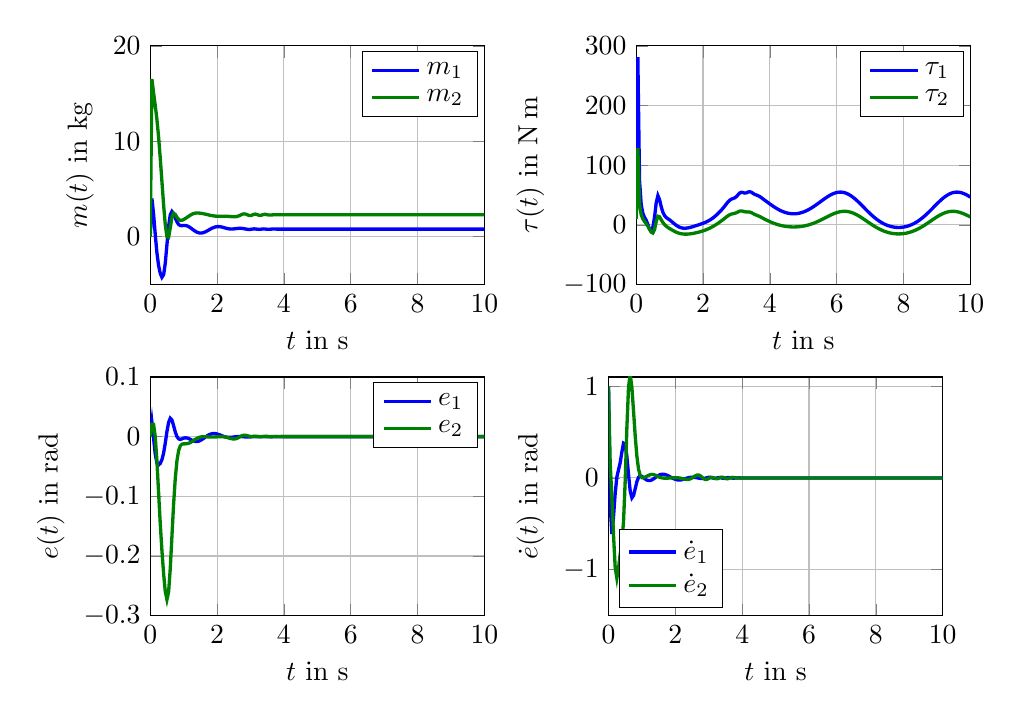
\begin{tikzpicture}

\begin{axis}[%
width=0.35\textwidth,
height=0.25\textwidth,
scale only axis,
xmin=0,
xmax=10,
xlabel={$t$ in $\mathrm{s}$},
xmajorgrids,
ymin=-1.5,
ymax=1.1,
ylabel={$\dot{e}(t)$ in $\mathrm{rad}$},
ymajorgrids,
name=plot1,
legend style={at={(0.03,0.03)},anchor=south west,draw=black,fill=white,legend cell align=left}
]
\addplot [
color=blue,
solid,
line width=1.2pt
]
table[row sep=crcr]{
0 1\\
0.05 -0.290087189677541\\
0.1 -0.610488735332477\\
0.15 -0.425110516326268\\
0.2 -0.168345383178169\\
0.25 0.0087426973931316\\
0.3 0.0894937430750705\\
0.35 0.166372312937989\\
0.4 0.281762661601077\\
0.45 0.378294580887595\\
0.5 0.367835109853427\\
0.55 0.234872203536229\\
0.6 0.0339819719259129\\
0.65 -0.143303327008248\\
0.7 -0.216974258992555\\
0.75 -0.190474066649986\\
0.8 -0.115554619262113\\
0.85 -0.0405415779761682\\
0.9 0.00739886464881667\\
0.95 0.0235306615881532\\
1 0.0175986054441741\\
1.05 0.00251040708171502\\
1.1 -0.0126505445090147\\
1.15 -0.0235309137354633\\
1.2 -0.0286235944797412\\
1.25 -0.0276313019138628\\
1.3 -0.0209533246432311\\
1.35 -0.00979403904121842\\
1.4 0.00383255751803424\\
1.45 0.0175043440656809\\
1.5 0.0290244385271177\\
1.55 0.0369280786482047\\
1.6 0.0406330305709996\\
1.65 0.0402647643576503\\
1.7 0.0363624848652983\\
1.75 0.0296564305546549\\
1.8 0.0209725473556486\\
1.85 0.0112097965572502\\
1.9 0.00131640733770222\\
1.95 -0.00776737929137417\\
2 -0.0151917464230467\\
2.05 -0.0202841123980473\\
2.1 -0.022626453743915\\
2.15 -0.0221171294649154\\
2.2 -0.0190106670330129\\
2.25 -0.0139210302932608\\
2.3 -0.00776551001839343\\
2.35 -0.00162900972674063\\
2.4 0.0034461718314317\\
2.45 0.0066940997858933\\
2.5 0.00779473253219842\\
2.55 0.00690491959362627\\
2.6 0.00454443924922665\\
2.65 0.00140199860431856\\
2.7 -0.00183818058728591\\
2.75 -0.00453679719256217\\
2.8 -0.00597800343304111\\
2.85 -0.00534255741515322\\
2.9 -0.00217371841210634\\
2.95 0.00273051483960596\\
3 0.00677481801120938\\
3.05 0.00664089938749202\\
3.1 0.00159522409998214\\
3.15 -0.00410245416311739\\
3.2 -0.00465898180022306\\
3.25 0.000517420819713954\\
3.3 0.00540973772260267\\
3.35 0.00411687030061236\\
3.4 -0.00173942562071927\\
3.45 -0.0050296912639437\\
3.5 -0.00226759980873881\\
3.55 0.00268066397579347\\
3.6 0.00424746042128044\\
3.65 0.00166050734593526\\
3.7 -0.0015027420045961\\
3.75 -0.00231898999252\\
3.8 -0.00110332507385613\\
3.85 0.000228603398043203\\
3.9 0.000608492710109765\\
3.95 0.00031755685394641\\
4 1.47161546079078e-05\\
4.05 -3.72110094878364e-05\\
4.1 4.38412486643003e-05\\
4.15 9.3757646349224e-05\\
4.2 7.383388894322e-05\\
4.25 3.00254677893519e-05\\
4.3 4.37980845163777e-06\\
4.35 2.50664100348574e-06\\
4.4 9.86868084423831e-06\\
4.45 1.42872136027483e-05\\
4.5 1.3398130703085e-05\\
4.55 1.04608336424783e-05\\
4.6 8.56110410712985e-06\\
4.65 8.32368380104115e-06\\
4.7 8.69038065587011e-06\\
4.75 8.46655037264887e-06\\
4.8 7.16140627204931e-06\\
4.85 4.95733778993479e-06\\
4.9 2.29861126133102e-06\\
4.95 -4.38088366749856e-07\\
5 -3.03144056662541e-06\\
5.05 -5.34185232797801e-06\\
5.1 -7.2207457870177e-06\\
5.15 -8.48488067828335e-06\\
5.2 -8.94981728827293e-06\\
5.25 -8.47354901534203e-06\\
5.3 -6.97537108895752e-06\\
5.35 -4.43451777898396e-06\\
5.4 -8.98632072976469e-07\\
5.45 3.47303801973009e-06\\
5.5 8.33274130285222e-06\\
5.55 1.30639270258248e-05\\
5.6 1.67534832906657e-05\\
5.65 1.82921424538574e-05\\
5.7 1.66726482384583e-05\\
5.75 1.14804457531648e-05\\
5.8 3.40286104538734e-06\\
5.85 -5.60664535320665e-06\\
5.9 -1.28708114036646e-05\\
5.95 -1.62009359846449e-05\\
6 -1.50964837141165e-05\\
6.05 -1.1000185181187e-05\\
6.1 -6.34123952114596e-06\\
6.15 -3.13446501598591e-06\\
6.2 -2.11777021830173e-06\\
6.25 -2.70098842047872e-06\\
6.3 -3.50320271991222e-06\\
6.35 -3.28982407815648e-06\\
6.4 -1.8766535337944e-06\\
6.45 -2.17405883851107e-07\\
6.5 5.29430184248447e-07\\
6.55 5.18666637416842e-08\\
6.6 -9.66045909600588e-07\\
6.65 -1.58089744306533e-06\\
6.7 -1.36337939038444e-06\\
6.75 -5.61888677141908e-07\\
6.8 2.71081074032509e-07\\
6.85 7.25120654410105e-07\\
6.9 7.1994139894116e-07\\
6.95 4.23709475505518e-07\\
7 6.88246981628282e-08\\
7.05 -1.84806733360965e-07\\
7.1 -2.89442572354304e-07\\
7.15 -2.79519771106962e-07\\
7.2 -2.20453910348972e-07\\
7.25 -1.69208779543517e-07\\
7.3 -1.5654732787862e-07\\
7.35 -1.86272271662791e-07\\
7.4 -2.42847562781368e-07\\
7.45 -3.01063935559398e-07\\
7.5 -3.34897900078346e-07\\
7.55 -3.24719120425865e-07\\
7.6 -2.62279008955701e-07\\
7.65 -1.52604222120045e-07\\
7.7 -1.2201872456874e-08\\
7.75 1.35874911807998e-07\\
7.8 2.68276042388049e-07\\
7.85 3.66654926360448e-07\\
7.9 4.20494016516171e-07\\
7.95 4.2728980288731e-07\\
8 3.91008109640323e-07\\
8.05 3.19989688302158e-07\\
8.1 2.25088722161093e-07\\
8.15 1.18262225401455e-07\\
8.2 1.14831606445875e-08\\
8.25 -8.42081707697062e-08\\
8.3 -1.59607874583578e-07\\
8.35 -2.08196050122123e-07\\
8.4 -2.26845561335232e-07\\
8.45 -2.1626083701598e-07\\
8.5 -1.80986002629169e-07\\
8.55 -1.28836527002463e-07\\
8.6 -6.97019844064783e-08\\
8.65 -1.38441903496656e-08\\
8.7 2.99753216692622e-08\\
8.75 5.60644262126431e-08\\
8.8 6.26273940484978e-08\\
8.85 5.16458840138512e-08\\
8.9 2.79387440960122e-08\\
8.95 -2.1968211694201e-09\\
9 -3.21433238914537e-08\\
9.05 -5.51590753072873e-08\\
9.1 -6.3453513776679e-08\\
9.15 -4.83928556116453e-08\\
9.2 -6.49921039208579e-09\\
9.25 4.86481007699879e-08\\
9.3 8.24342484273544e-08\\
9.35 6.19894647835295e-08\\
9.4 -3.64121865992217e-09\\
9.45 -5.51732229903124e-08\\
9.5 -3.87181752214971e-08\\
9.55 2.68918077805935e-08\\
9.6 6.34046367631314e-08\\
9.65 2.65209439964664e-08\\
9.7 -3.80852613890426e-08\\
9.75 -5.38315099163356e-08\\
9.8 -8.46103287432953e-09\\
9.85 3.96475897668225e-08\\
9.9 4.03954149019725e-08\\
9.95 4.74649142212513e-09\\
10 -2.39542836677487e-08\\
};
\addlegendentry{$\dot{e}_1$};

\addplot [
color=green!50!black,
solid,
line width=1.2pt
]
table[row sep=crcr]{
0 1\\
0.05 0.166027864776492\\
0.1 -0.199734651209782\\
0.15 -0.621527276148698\\
0.2 -0.975204912711275\\
0.25 -1.09099303622838\\
0.3 -0.981180061366164\\
0.35 -0.830670822728419\\
0.4 -0.699751488433112\\
0.45 -0.472839183720434\\
0.5 -0.0297201566176722\\
0.55 0.545996179684783\\
0.6 0.9958528587681\\
0.65 1.12787238655081\\
0.7 0.986727686260749\\
0.75 0.724011500716038\\
0.8 0.452437301442763\\
0.85 0.234309454320129\\
0.9 0.0940008550335687\\
0.95 0.0246611045535359\\
1 0.00204812905841423\\
1.05 0.00201074986612654\\
1.1 0.00980780686837646\\
1.15 0.0193680991462767\\
1.2 0.0285444745156288\\
1.25 0.0356228160961983\\
1.3 0.0386547723839966\\
1.35 0.0365200024477139\\
1.4 0.0298568875900593\\
1.45 0.0208245740091555\\
1.5 0.0119520350055893\\
1.55 0.00499855033983137\\
1.6 0.000523980854993715\\
1.65 -0.0018025236753941\\
1.7 -0.00261245112978359\\
1.75 -0.00242446811315278\\
1.8 -0.0015553742643456\\
1.85 -0.000233251087416508\\
1.9 0.00126904303135122\\
1.95 0.00257828344491629\\
2 0.00324982626413028\\
2.05 0.00285173179049153\\
2.1 0.00107837628566365\\
2.15 -0.00212488224035423\\
2.2 -0.00644957412071745\\
2.25 -0.0111615344311411\\
2.3 -0.0151348388643907\\
2.35 -0.017021787429871\\
2.4 -0.0155631952099594\\
2.45 -0.00999006024859217\\
2.5 -0.000434321961879869\\
2.55 0.0117275223902267\\
2.6 0.0237070275937508\\
2.65 0.0316136795660157\\
2.7 0.0317176956491643\\
2.75 0.0226416319679343\\
2.8 0.00714146896107204\\
2.85 -0.00838553577183199\\
2.9 -0.0169879987489253\\
2.95 -0.0152583810945279\\
3 -0.00598955983194394\\
3.05 0.00329005429663976\\
3.1 0.00596704609914456\\
3.15 0.00118771199697898\\
3.2 -0.00616988149484232\\
3.25 -0.00920331032572541\\
3.3 -0.00436290214986357\\
3.35 0.00452955006520228\\
3.4 0.0089134521387908\\
3.45 0.00421087751801119\\
3.5 -0.00497766879674832\\
3.55 -0.00964494394939064\\
3.6 -0.00589734238828166\\
3.65 0.00166031859220406\\
3.7 0.00602798502397772\\
3.75 0.00495917207786023\\
3.8 0.00136112147975276\\
3.85 -0.00116119399278092\\
3.9 -0.00154600326483478\\
3.95 -0.000861696347391527\\
4 -0.000313337896954979\\
4.05 -0.000219477358408327\\
4.1 -0.000307431173514949\\
4.15 -0.000316075350742184\\
4.2 -0.000216679733501868\\
4.25 -0.000100220011689967\\
4.3 -3.06001211997642e-05\\
4.35 -7.0154418279067e-06\\
4.4 -3.87954120439904e-07\\
4.45 9.43358388644233e-06\\
4.5 2.47941691424447e-05\\
4.55 3.94669198258424e-05\\
4.6 4.85660947414507e-05\\
4.65 5.17047488306221e-05\\
4.7 5.11400736328514e-05\\
4.75 4.90643230050686e-05\\
4.8 4.63623932332735e-05\\
4.85 4.28636809486904e-05\\
4.9 3.81215780184407e-05\\
4.95 3.19351821057579e-05\\
5 2.44094613281454e-05\\
5.05 1.57551582852244e-05\\
5.1 6.10046790483487e-06\\
5.15 -4.55342907418332e-06\\
5.2 -1.62600466370177e-05\\
5.25 -2.90273170669986e-05\\
5.3 -4.27396794799861e-05\\
5.35 -5.70838040275801e-05\\
5.4 -7.14302433463265e-05\\
5.45 -8.46566619917555e-05\\
5.5 -9.49699879776444e-05\\
5.55 -9.98607367275195e-05\\
5.6 -9.63795468483797e-05\\
5.65 -8.19270666680971e-05\\
5.7 -5.5607524044432e-05\\
5.75 -1.9810349589755e-05\\
5.8 1.89038456288593e-05\\
5.85 5.09086288814631e-05\\
5.9 6.72826025130968e-05\\
5.95 6.48804058148711e-05\\
6 4.90593576564224e-05\\
6.05 3.07593514484727e-05\\
6.1 1.9110043334658e-05\\
6.15 1.57079774152358e-05\\
6.2 1.57582978764781e-05\\
6.25 1.41941953256675e-05\\
6.3 1.00592337187733e-05\\
6.35 5.67260219319632e-06\\
6.4 3.25775154608188e-06\\
6.45 3.06484457746059e-06\\
6.5 3.86857766043747e-06\\
6.55 4.29615710262343e-06\\
6.6 3.67032262726941e-06\\
6.65 2.14052335245629e-06\\
6.7 3.70030697194323e-07\\
6.75 -9.29707650421108e-07\\
6.8 -1.37100871799856e-06\\
6.85 -1.00775699962696e-06\\
6.9 -2.01921725673238e-07\\
6.95 6.19496871911984e-07\\
7 1.15850108373117e-06\\
7.05 1.31528404989645e-06\\
7.1 1.15029017855317e-06\\
7.15 8.00945400891706e-07\\
7.2 4.0740648554749e-07\\
7.25 7.15881850466005e-08\\
7.3 -1.52523071283994e-07\\
7.35 -2.51019323882495e-07\\
7.4 -2.37688991100438e-07\\
7.45 -1.4362196415485e-07\\
7.5 -9.185552707347e-09\\
7.55 1.23790789063882e-07\\
7.6 2.20605293643761e-07\\
7.65 2.6131439911925e-07\\
7.7 2.44236647128915e-07\\
7.75 1.83455039520775e-07\\
7.8 1.01509114558418e-07\\
7.85 2.08871301487362e-08\\
7.9 -4.20550829438593e-08\\
7.95 -7.9203918923465e-08\\
8 -8.96475511047434e-08\\
8.05 -7.73744938953325e-08\\
8.1 -4.91787670309218e-08\\
8.15 -1.32250870255035e-08\\
8.2 2.19641620446964e-08\\
8.25 4.84467462813498e-08\\
8.3 5.98613280056171e-08\\
8.35 5.24246677180429e-08\\
8.4 2.57702048589437e-08\\
8.45 -1.65464433266038e-08\\
8.5 -6.70523871981743e-08\\
8.55 -1.15029288760837e-07\\
8.6 -1.47932588401289e-07\\
8.65 -1.53511651501681e-07\\
8.7 -1.22472251118388e-07\\
8.75 -5.14997302580866e-08\\
8.8 5.35357401743042e-08\\
8.85 1.74700232724589e-07\\
8.9 2.81138548996474e-07\\
8.95 3.33797828044879e-07\\
9 2.99578652551702e-07\\
9.05 1.73450532381381e-07\\
9.1 -4.45532433168694e-09\\
9.15 -1.57371018882912e-07\\
9.2 -2.13717565311633e-07\\
9.25 -1.57333509553936e-07\\
9.3 -4.22800559007896e-08\\
9.35 4.57127504738253e-08\\
9.4 5.062289309965e-08\\
9.45 -1.69696767748917e-08\\
9.5 -9.0020907395072e-08\\
9.55 -9.56761075920909e-08\\
9.6 -1.85073418812465e-08\\
9.65 7.54524970281167e-08\\
9.7 9.46956393299558e-08\\
9.75 1.79152066515087e-08\\
9.8 -7.80749558337845e-08\\
9.85 -1.00276861592086e-07\\
9.9 -3.69189842031048e-08\\
9.95 4.26882731385803e-08\\
10 7.18547878975073e-08\\
};
\addlegendentry{$\dot{e}_2$};

\end{axis}

\begin{axis}[%
width=0.35\textwidth,
height=0.25\textwidth,
scale only axis,
xmin=0,
xmax=10,
xlabel={$t$ in $\mathrm{s}$},
xmajorgrids,
ymin=-0.3,
ymax=0.1,
ylabel={$e(t)$ in $\mathrm{rad}$},
ymajorgrids,
name=plot3,
at=(plot1.left of south west),
anchor=right of south east,
legend style={draw=black,fill=white,legend cell align=left}
]
\addplot [
color=blue,
solid,
line width=1.2pt
]
table[row sep=crcr]{
0 0\\
0.05 0.0241513685447209\\
0.1 -0.00266980595040972\\
0.15 -0.0293114871648896\\
0.2 -0.0440623402696887\\
0.25 -0.0475516540004715\\
0.3 -0.0448696946353956\\
0.35 -0.0386259198475413\\
0.4 -0.0275284610061786\\
0.45 -0.0107417813989652\\
0.5 0.00846561399285467\\
0.55 0.0239607957126293\\
0.6 0.0308008306330075\\
0.65 0.0277524734253705\\
0.7 0.0182566249562275\\
0.75 0.0077502105249706\\
0.8 1.16275628002649e-05\\
0.85 -0.00381626045299466\\
0.9 -0.00450685602949619\\
0.95 -0.00361482626064935\\
1 -0.0025229019329881\\
1.05 -0.00200498457703069\\
1.1 -0.00227027439715233\\
1.15 -0.00319715772167739\\
1.2 -0.0045263206055971\\
1.25 -0.00595775641984142\\
1.3 -0.00719422985707752\\
1.35 -0.00797791835763206\\
1.4 -0.00813226799719868\\
1.45 -0.00759404458906077\\
1.5 -0.00641812852179491\\
1.55 -0.00475238878272699\\
1.6 -0.00279569955258852\\
1.65 -0.000757196221737644\\
1.7 0.00117178013609653\\
1.75 0.00283227434745637\\
1.8 0.00410441811837414\\
1.85 0.00491151782958654\\
1.9 0.00522322306215128\\
1.95 0.00505670192046892\\
2 0.00447424124417695\\
2.05 0.00357653634681221\\
2.1 0.00249184084308363\\
2.15 0.00136161889450892\\
2.2 0.000323617146759103\\
2.25 -0.000506220856337003\\
2.3 -0.00105062257064636\\
2.35 -0.00128311048994445\\
2.4 -0.00123137009466079\\
2.45 -0.000969205254074845\\
2.5 -0.000598023780444934\\
2.55 -0.000223113361896732\\
2.6 6.78643193606776e-05\\
2.65 0.000218309528336957\\
2.7 0.000206474431026171\\
2.75 4.34717197380086e-05\\
2.8 -0.000226344366438203\\
2.85 -0.000519552810157475\\
2.9 -0.000717661667709507\\
2.95 -0.000706896728199569\\
3 -0.000458348504592032\\
3.05 -0.000100498322940484\\
3.1 0.000120607050927944\\
3.15 4.70009372187819e-05\\
3.2 -0.000200626681248407\\
3.25 -0.000319019006123702\\
3.3 -0.000153581094299082\\
3.35 0.000113898152631631\\
3.4 0.000178361545092653\\
3.45 -1.47563566409992e-05\\
3.5 -0.000218870367839574\\
3.55 -0.000204095090262646\\
3.6 -1.0425178735729e-05\\
3.65 0.000148648644969773\\
3.7 0.000146623531760426\\
3.75 3.96336077269632e-05\\
3.8 -5.04835345080945e-05\\
3.85 -6.94034271917499e-05\\
3.9 -4.43490794690415e-05\\
3.95 -1.99144483350455e-05\\
4 -1.25070330073696e-05\\
4.05 -1.40298617907764e-05\\
4.1 -1.40025513327702e-05\\
4.15 -1.02503522709796e-05\\
4.2 -5.83973111056846e-06\\
4.25 -3.25772653697598e-06\\
4.3 -2.51063519118855e-06\\
4.35 -2.41217920005088e-06\\
4.4 -2.10855712401425e-06\\
4.45 -1.48056280246944e-06\\
4.5 -7.71382950515154e-07\\
4.55 -1.74428668731075e-07\\
4.6 2.93640826987129e-07\\
4.65 7.10418205818186e-07\\
4.7 1.1361463969628e-06\\
4.75 1.56921027194556e-06\\
4.8 1.96442950817222e-06\\
4.85 2.27027750954178e-06\\
4.9 2.45268427623291e-06\\
4.95 2.49897685311584e-06\\
5 2.41134862766224e-06\\
5.05 2.20057496957971e-06\\
5.1 1.88436736381359e-06\\
5.15 1.48878001005048e-06\\
5.2 1.04925923516408e-06\\
5.25 6.09554838604254e-07\\
5.3 2.1900303848188e-07\\
5.35 -7.05341398621329e-08\\
5.4 -2.07769819238202e-07\\
5.45 -1.46326752936687e-07\\
5.5 1.47858288945812e-07\\
5.55 6.85017842894098e-07\\
5.6 1.43705390909243e-06\\
5.65 2.32451786752463e-06\\
5.7 3.2133499623388e-06\\
5.75 3.93164756873343e-06\\
5.8 4.31259569849685e-06\\
5.85 4.25599264280985e-06\\
5.9 3.78133318679197e-06\\
5.95 3.0355297793716e-06\\
6 2.23636184026876e-06\\
6.05 1.57635965064573e-06\\
6.1 1.14547148585831e-06\\
6.15 9.17281167051032e-07\\
6.2 7.94755127916935e-07\\
6.25 6.78361486795842e-07\\
6.3 5.21058459303225e-07\\
6.35 3.45570654994298e-07\\
6.4 2.12729140677825e-07\\
6.45 1.62055223712487e-07\\
6.5 1.75148794662183e-07\\
6.55 1.93867595310593e-07\\
6.6 1.71074417076866e-07\\
6.65 1.04195584382794e-07\\
6.7 2.71478300950534e-08\\
6.75 -2.23674935795337e-08\\
6.8 -2.87476926708052e-08\\
6.85 -1.90970117497358e-09\\
6.9 3.5835595713074e-08\\
6.95 6.50735134666292e-08\\
7 7.71506638574948e-08\\
7.05 7.35883263214276e-08\\
7.1 6.10818707835747e-08\\
7.15 4.64557867729809e-08\\
7.2 3.38336443306275e-08\\
7.25 2.41602527983886e-08\\
7.3 1.61551682031913e-08\\
7.35 7.69431063307735e-09\\
7.4 -3.01368674460178e-09\\
7.45 -1.67018970875787e-08\\
7.5 -3.27887887952016e-08\\
7.55 -4.95255196852895e-08\\
7.6 -6.44512334613268e-08\\
7.65 -7.50242121760891e-08\\
7.7 -7.9256083473922e-08\\
7.75 -7.61725433839899e-08\\
7.8 -6.59850563078379e-08\\
7.85 -4.99651112706445e-08\\
7.9 -3.01116882539532e-08\\
7.95 -8.74553107710341e-09\\
8 1.18575668173193e-08\\
8.05 2.97380802205538e-08\\
8.1 4.34231530732632e-08\\
8.15 5.20152488858727e-08\\
8.2 5.52192044311894e-08\\
8.25 5.33190158691355e-08\\
8.3 4.71084766751062e-08\\
8.35 3.77778015536734e-08\\
8.4 2.67608907256189e-08\\
8.45 1.55532787760038e-08\\
8.5 5.51821499605865e-09\\
8.55 -2.29371954763025e-09\\
8.6 -7.28076887668294e-09\\
8.65 -9.35271948776517e-09\\
8.7 -8.90246087958957e-09\\
8.75 -6.68945243642582e-09\\
8.8 -3.66181396316279e-09\\
8.85 -7.60526530640959e-10\\
8.9 1.24869137252404e-09\\
8.95 1.88392434985474e-09\\
9 9.89629822534255e-10\\
9.05 -1.25760712954559e-09\\
9.1 -4.32226765489929e-09\\
9.15 -7.24872467605664e-09\\
9.2 -8.73675704005095e-09\\
9.25 -7.68906699422089e-09\\
9.3 -4.2426616664315e-09\\
9.35 -3.78328771089009e-10\\
9.4 1.18100162982415e-09\\
9.45 -4.7863119717606e-10\\
9.5 -3.11174375156043e-09\\
9.55 -3.42925138285821e-09\\
9.6 -8.50611581171279e-10\\
9.65 1.72211572779801e-09\\
9.7 1.42634287714216e-09\\
9.75 -1.11075437736474e-09\\
9.8 -2.7656256174069e-09\\
9.85 -1.78614806278787e-09\\
9.9 5.05097463854298e-10\\
9.95 1.76517400696241e-09\\
10 1.24982801885665e-09\\
};
\addlegendentry{$e_1$};

\addplot [
color=green!50!black,
solid,
line width=1.2pt
]
table[row sep=crcr]{
0 0\\
0.05 0.0205943320514263\\
0.1 0.0203180473559811\\
0.15 -0.000200748910283738\\
0.2 -0.0407717544609035\\
0.25 -0.0936281971422599\\
0.3 -0.145987060198247\\
0.35 -0.191165213629595\\
0.4 -0.229490813002331\\
0.45 -0.259549917994451\\
0.5 -0.273035769572548\\
0.55 -0.260200622701998\\
0.6 -0.220571535809602\\
0.65 -0.166076277504419\\
0.7 -0.112391563518184\\
0.75 -0.0693967501621412\\
0.8 -0.0401102362263753\\
0.85 -0.0232418123963236\\
0.9 -0.0153641881311807\\
0.95 -0.0126489176975193\\
1 -0.0121200457384044\\
1.05 -0.0120738234165833\\
1.1 -0.0117934532108098\\
1.15 -0.0110657088071938\\
1.2 -0.00986306737783871\\
1.25 -0.008245976229594\\
1.3 -0.00636870457755889\\
1.35 -0.00446768052050883\\
1.4 -0.00279308896867636\\
1.45 -0.00152167970066419\\
1.5 -0.000707485911490613\\
1.55 -0.000293771125304154\\
1.6 -0.000165802439459295\\
1.65 -0.000205420346707341\\
1.7 -0.000320865520212932\\
1.75 -0.000450159376776504\\
1.8 -0.000552009816014332\\
1.85 -0.000598115087511508\\
1.9 -0.000572270256327556\\
1.95 -0.000474384980816533\\
2 -0.000325075269608233\\
2.05 -0.000167298898685275\\
2.1 -6.29631162859523e-05\\
2.15 -8.34977998372954e-05\\
2.2 -0.000294384791720059\\
2.25 -0.000735136684142379\\
2.3 -0.00139836040877528\\
2.35 -0.00221380523648163\\
2.4 -0.00304450816532342\\
2.45 -0.00370104397211646\\
2.5 -0.00397643633770839\\
2.55 -0.00370022815690929\\
2.6 -0.00280604365269399\\
2.65 -0.00139741718373404\\
2.7 0.000223955668186171\\
2.75 0.00161888351661732\\
2.8 0.00237883251773013\\
2.85 0.00233220339623486\\
2.9 0.00165774409979724\\
2.95 0.000809342998040363\\
3 0.000260545194271877\\
3.05 0.000209993574090739\\
3.1 0.000475899448106089\\
3.15 0.000679012491959325\\
3.2 0.000550459053153866\\
3.25 0.000135992084095551\\
3.3 -0.000234038965679279\\
3.35 -0.000229589557220661\\
3.4 0.000141278945681611\\
3.45 0.000504407004974172\\
3.5 0.000484764945014315\\
3.55 8.53314802046201e-05\\
3.6 -0.000333965534274616\\
3.65 -0.000439522290058614\\
3.7 -0.000224322865794879\\
3.75 6.94412758027729e-05\\
3.8 0.000229185705520552\\
3.85 0.000225192561224552\\
3.9 0.00014997935896488\\
3.95 8.83915891415343e-05\\
4 6.09493370465897e-05\\
4.05 4.91402559339438e-05\\
4.1 3.60118849871416e-05\\
4.15 1.98718924062646e-05\\
4.2 6.2710316137693e-06\\
4.25 -1.53627206045392e-06\\
4.3 -4.57295400768665e-06\\
4.35 -5.37892554519637e-06\\
4.4 -5.55009955494068e-06\\
4.45 -5.35359907505306e-06\\
4.5 -4.50997699774636e-06\\
4.55 -2.88715102803039e-06\\
4.6 -6.59227547550323e-07\\
4.65 1.86842603555615e-06\\
4.7 4.4495031977787e-06\\
4.75 6.95791193205952e-06\\
4.8 9.3459550351005e-06\\
4.85 1.15808479830282e-05\\
4.9 1.36112843684977e-05\\
4.95 1.53686106804107e-05\\
5 1.67822961519848e-05\\
5.05 1.77906835439057e-05\\
5.1 1.83411039365033e-05\\
5.15 1.83840012333292e-05\\
5.2 1.78680866692593e-05\\
5.25 1.67401539529211e-05\\
5.3 1.49494059599187e-05\\
5.35 1.24553992535414e-05\\
5.4 9.24063161011901e-06\\
5.45 5.3305823308758e-06\\
5.5 8.23022133111806e-07\\
5.55 -4.07639250354919e-06\\
5.6 -9.02343608943923e-06\\
5.65 -1.35306351873865e-05\\
5.7 -1.70165574270298e-05\\
5.75 -1.89310347893379e-05\\
5.8 -1.89471315508172e-05\\
5.85 -1.71528040205371e-05\\
5.9 -1.4120193041145e-05\\
5.95 -1.07426695543089e-05\\
6 -7.85929219299097e-06\\
6.05 -5.87694052989196e-06\\
6.1 -4.66777651156325e-06\\
6.15 -3.82451029656838e-06\\
6.2 -3.03939222699723e-06\\
6.25 -2.27820822690239e-06\\
6.3 -1.66469409798933e-06\\
6.35 -1.27611980704767e-06\\
6.4 -1.06308941071054e-06\\
6.45 -9.12208581227425e-07\\
6.5 -7.39688928108606e-07\\
6.55 -5.31760050825891e-07\\
6.6 -3.27797390453632e-07\\
6.65 -1.79750493045638e-07\\
6.7 -1.17424896695084e-07\\
6.75 -1.3434304063642e-07\\
6.8 -1.95460594487606e-07\\
6.85 -2.57491066246729e-07\\
6.9 -2.88464906073038e-07\\
6.95 -2.77145736693463e-07\\
7 -2.30987309723929e-07\\
7.05 -1.67413306662034e-07\\
7.1 -1.04528211197774e-07\\
7.15 -5.51304346618764e-08\\
7.2 -2.48321743168134e-08\\
7.25 -1.30966503197882e-08\\
7.3 -1.54973512911383e-08\\
7.35 -2.59602915830826e-08\\
7.4 -3.84581153589636e-08\\
7.45 -4.81223924042595e-08\\
7.5 -5.19024122569434e-08\\
7.55 -4.88368127049554e-08\\
7.6 -3.9913546467929e-08\\
7.65 -2.75122410409168e-08\\
7.7 -1.45555931752028e-08\\
7.75 -3.63368568567779e-09\\
7.8 3.6151199811485e-09\\
7.85 6.71074995572951e-09\\
7.9 6.16146167420339e-09\\
7.95 3.08817649230519e-09\\
8 -1.17096876639522e-09\\
8.05 -5.3646446174227e-09\\
8.1 -8.51841430726807e-09\\
8.15 -1.00366013278119e-08\\
8.2 -9.74455727220658e-09\\
8.25 -7.88327492173835e-09\\
8.3 -5.05559483165996e-09\\
8.35 -2.12192496906738e-09\\
8.4 -4.93555196712236e-11\\
8.45 2.73573275144656e-10\\
8.5 -1.7646685224193e-09\\
8.55 -6.31650032278941e-09\\
8.6 -1.29453255892642e-08\\
8.65 -2.05845894774015e-08\\
8.7 -2.76171815416504e-08\\
8.75 -3.20976806245099e-08\\
8.8 -3.21312874085322e-08\\
8.85 -2.6408631503827e-08\\
8.9 -1.48448923154021e-08\\
8.95 8.59657511842471e-10\\
9 1.71202738652454e-08\\
9.05 2.93021735209287e-08\\
9.1 3.36148040513962e-08\\
9.15 2.92997271444939e-08\\
9.2 1.95306442685173e-08\\
9.25 9.8411549465105e-09\\
9.3 4.76191308607099e-09\\
9.35 5.08254908992978e-09\\
9.4 7.81379762629375e-09\\
9.45 8.77134266261126e-09\\
9.5 5.85193651869709e-09\\
9.55 7.18775872154964e-10\\
9.6 -2.52879625572966e-09\\
9.65 -1.11278236625267e-09\\
9.7 3.41969608186332e-09\\
9.75 6.36203667525592e-09\\
9.8 4.53194282101776e-09\\
9.85 -5.24135845836327e-10\\
9.9 -4.38804143021443e-09\\
9.95 -4.32325186761062e-09\\
10 -1.37613631601141e-09\\
};
\addlegendentry{$e_2$};

\end{axis}

\begin{axis}[%
width=0.35\textwidth,
height=0.25\textwidth,
scale only axis,
xmin=0,
xmax=10,
xlabel={$t$ in $\mathrm{s}$},
xmajorgrids,
ymin=-5,
ymax=20,
ylabel={$m(t)$ in $\mathrm{kg}$},
ymajorgrids,
name=plot2,
at=(plot3.above north west),
anchor=below south west,
legend style={draw=black,fill=white,legend cell align=left}
]
\addplot [
color=blue,
solid,
line width=1.2pt
]
table[row sep=crcr]{
0 0\\
0.05 4.01631231308313\\
0.1 2.37135913602382\\
0.15 0.239144461351218\\
0.2 -1.67309394861457\\
0.25 -3.01191584483333\\
0.3 -3.84496316651013\\
0.35 -4.24917551135839\\
0.4 -3.98158868712329\\
0.45 -2.76813641269678\\
0.5 -0.826130528638791\\
0.55 1.09143120845056\\
0.6 2.30546471272078\\
0.65 2.64678689604048\\
0.7 2.41134581513947\\
0.75 1.96766203334831\\
0.8 1.55325789103299\\
0.85 1.28404607923852\\
0.9 1.17371516693481\\
0.95 1.16504763675551\\
1 1.18458204940891\\
1.05 1.18292556657168\\
1.1 1.14132329299213\\
1.15 1.06048890070418\\
1.2 0.949854159569933\\
1.25 0.822219657292584\\
1.3 0.69166686490254\\
1.35 0.572218623721803\\
1.4 0.476283369945058\\
1.45 0.413020373696154\\
1.5 0.387163189981492\\
1.55 0.398758409729696\\
1.6 0.443852942922116\\
1.65 0.515700263143948\\
1.7 0.605946720597064\\
1.75 0.705534973781528\\
1.8 0.805384314053539\\
1.85 0.897006373988132\\
1.9 0.973120825301917\\
1.95 1.02822584861921\\
2 1.05905195985725\\
2.05 1.0648599573192\\
2.1 1.04756736104841\\
2.15 1.0116699672906\\
2.2 0.963881094263941\\
2.25 0.912385479064917\\
2.3 0.86565269260093\\
2.35 0.830913408789854\\
2.4 0.81263807736708\\
2.45 0.811529580928657\\
2.5 0.824462847629484\\
2.55 0.845433387463631\\
2.6 0.867134136419907\\
2.65 0.882572546334021\\
2.7 0.886285519936806\\
2.75 0.875170595665262\\
2.8 0.849524796216918\\
2.85 0.814695097597237\\
2.9 0.782003638792098\\
2.95 0.765884063725233\\
3 0.775318221441698\\
3.05 0.803163105276294\\
3.1 0.825460638491265\\
3.15 0.820893573740939\\
3.2 0.794767575558628\\
3.25 0.776178190908029\\
3.3 0.786166180904195\\
3.35 0.81217485312115\\
3.4 0.822690210195948\\
3.45 0.806318423068133\\
3.5 0.783639419160515\\
3.55 0.779496741462272\\
3.6 0.795007464319672\\
3.65 0.811587184856813\\
3.7 0.815081443165755\\
3.75 0.807717751571058\\
3.8 0.799618146484244\\
3.85 0.796590206786304\\
3.9 0.79746018230212\\
3.95 0.798828349925446\\
4 0.799123874980357\\
4.05 0.798751006148455\\
4.1 0.798479025167968\\
4.15 0.798528203220598\\
4.2 0.798704145991325\\
4.25 0.798810344634696\\
4.3 0.798814151611613\\
4.35 0.798779000909343\\
4.4 0.798760906765533\\
4.45 0.798772396667828\\
4.5 0.79880026266111\\
4.55 0.798831232577781\\
4.6 0.798862120161646\\
4.65 0.798896452179443\\
4.7 0.798937828735072\\
4.75 0.79898644431435\\
4.8 0.79903938567088\\
4.85 0.79909253965667\\
4.9 0.799142142223056\\
4.95 0.799185314104379\\
5 0.799219924880618\\
5.05 0.799244375941215\\
5.1 0.799257634807213\\
5.15 0.799259502382302\\
5.2 0.799250921407678\\
5.25 0.79923417574769\\
5.3 0.79921296122303\\
5.35 0.79919238044949\\
5.4 0.799178864090657\\
5.45 0.799179895928821\\
5.5 0.799203317302347\\
5.55 0.799255989775193\\
5.6 0.79934175614204\\
5.65 0.799459001247863\\
5.7 0.799598664976916\\
5.75 0.79974409079674\\
5.8 0.799874079055604\\
5.85 0.799969323305955\\
5.9 0.800020039981438\\
5.95 0.800030504887789\\
6 0.800016831173345\\
6.05 0.799998536485343\\
6.1 0.799989170415603\\
6.15 0.799991761144167\\
6.2 0.800000676617445\\
6.25 0.800007412503061\\
6.3 0.800006774955135\\
6.35 0.800000200843124\\
6.4 0.799993951493369\\
6.45 0.799993409891558\\
6.5 0.799998545665727\\
6.55 0.800004618938527\\
6.6 0.800006806303752\\
6.65 0.800003972319136\\
6.7 0.79999866530387\\
6.75 0.799994429908295\\
6.8 0.799993293462578\\
6.85 0.799995093198818\\
6.9 0.799998351250254\\
6.95 0.800001516785231\\
7 0.800003708700055\\
7.05 0.800004796020997\\
7.1 0.800005095232921\\
7.15 0.800005018142261\\
7.2 0.800004853249369\\
7.25 0.800004704930503\\
7.3 0.800004533989277\\
7.35 0.800004233883643\\
7.4 0.800003700381504\\
7.45 0.800002877653419\\
7.5 0.800001778739739\\
7.55 0.800000483997562\\
7.6 0.799999122839233\\
7.65 0.799997845418349\\
7.7 0.799996792226336\\
7.75 0.799996069374078\\
7.8 0.799995734730019\\
7.85 0.799995795889936\\
7.9 0.79999621716025\\
7.95 0.799996931006164\\
8 0.799997850004854\\
8.05 0.799998877224135\\
8.1 0.79999991475524\\
8.15 0.800000871050754\\
8.2 0.800001667724033\\
8.25 0.800002245969631\\
8.3 0.800002572183612\\
8.35 0.800002641916478\\
8.4 0.800002481057642\\
8.45 0.80000214319849\\
8.5 0.800001702554544\\
8.55 0.80000124270495\\
8.6 0.8000008426157\\
8.65 0.800000562590984\\
8.7 0.80000043340727\\
8.75 0.800000451457823\\
8.8 0.800000581210387\\
8.85 0.800000764185174\\
8.9 0.800000931883043\\
8.95 0.800001019384188\\
9 0.800000977176059\\
9.05 0.800000781627452\\
9.1 0.80000044833179\\
9.15 0.80000005029076\\
9.2 0.7999997243632\\
9.25 0.799999625426587\\
9.3 0.799999809863783\\
9.35 0.800000130348886\\
9.4 0.800000299616938\\
9.45 0.800000151587683\\
9.5 0.799999847310036\\
9.55 0.799999729407566\\
9.6 0.79999992771643\\
9.65 0.800000195726678\\
9.7 0.800000213076064\\
9.75 0.799999973930411\\
9.8 0.799999765021205\\
9.85 0.799999799608742\\
9.9 0.799999999165691\\
9.95 0.800000145425537\\
10 0.800000136674073\\
};
\addlegendentry{$m_1$};

\addplot [
color=green!50!black,
solid,
line width=1.2pt
]
table[row sep=crcr]{
0 0\\
0.05 16.5254788905806\\
0.1 15.0770527388076\\
0.15 13.7414934798822\\
0.2 12.2871206081222\\
0.25 10.4415730665857\\
0.3 8.23028852115849\\
0.35 5.78766045416228\\
0.4 3.34253294937773\\
0.45 1.27493283517074\\
0.5 0.0252524787686259\\
0.55 -0.0491721616951275\\
0.6 0.960059121752467\\
0.65 2.05981638151407\\
0.7 2.46512736957455\\
0.75 2.33096080580105\\
0.8 2.04161730272378\\
0.85 1.8166968522718\\
0.9 1.72000465327688\\
0.95 1.73123921232012\\
1 1.80567111564184\\
1.05 1.9093336673222\\
1.1 2.02582357741815\\
1.15 2.14681262220603\\
1.2 2.26272601669834\\
1.25 2.36143821565529\\
1.3 2.43303278680289\\
1.35 2.47436516119329\\
1.4 2.48924179816316\\
1.45 2.48480783928125\\
1.5 2.46749242293943\\
1.55 2.4411568686694\\
1.6 2.40770944108571\\
1.65 2.36871820986824\\
1.7 2.32648427651206\\
1.75 2.28405509773636\\
1.8 2.24458013465457\\
1.85 2.21062774205113\\
1.9 2.18379685248971\\
1.95 2.16463395795315\\
2 2.15273625813121\\
2.05 2.14694023997314\\
2.1 2.14554135936661\\
2.15 2.14651331764493\\
2.2 2.14770907901116\\
2.25 2.14705327427784\\
2.3 2.14278131151097\\
2.35 2.13383162083765\\
2.4 2.12051780345172\\
2.45 2.10551767731133\\
2.5 2.09489940078907\\
2.55 2.09829410147246\\
2.6 2.12664303826867\\
2.65 2.18612587050839\\
2.7 2.26953802386026\\
2.75 2.35156879507907\\
2.8 2.39669986521966\\
2.85 2.38058326211408\\
2.9 2.31221020029786\\
2.95 2.2384676360171\\
3 2.2181081577714\\
3.05 2.27111707420609\\
3.1 2.34836927556677\\
3.15 2.37365590619409\\
3.2 2.3242400764874\\
3.25 2.25461939950898\\
3.3 2.23759091025162\\
3.35 2.28564736290911\\
3.4 2.34054400166529\\
3.45 2.34645371111619\\
3.5 2.30950665281548\\
3.55 2.27552734959947\\
3.6 2.27291711253437\\
3.65 2.29122537389939\\
3.7 2.30596957575222\\
3.75 2.30751699802159\\
3.8 2.302628634382\\
3.85 2.29965667886798\\
3.9 2.30012433362604\\
3.95 2.30138164825999\\
4 2.30161151028758\\
4.05 2.301072305891\\
4.1 2.30063306682249\\
4.15 2.30060450601165\\
4.2 2.30077474582461\\
4.25 2.30089281063309\\
4.3 2.3009013470192\\
4.35 2.30086888448677\\
4.4 2.30085932718201\\
4.45 2.30088235748687\\
4.5 2.30091527346142\\
4.55 2.30093696786299\\
4.6 2.30094162977465\\
4.65 2.30093414361328\\
4.7 2.30092100191615\\
4.75 2.30090550570642\\
4.8 2.30088801270774\\
4.85 2.3008681862647\\
4.9 2.30084657530953\\
4.95 2.30082474470287\\
5 2.30080453541186\\
5.05 2.30078730432663\\
5.1 2.3007735749274\\
5.15 2.30076303281595\\
5.2 2.30075458631613\\
5.25 2.30074630121399\\
5.3 2.30073522696184\\
5.35 2.30071727747037\\
5.4 2.30068735919187\\
5.45 2.30063991303123\\
5.5 2.30057001693661\\
5.55 2.30047514651111\\
5.6 2.30035747708058\\
5.65 2.30022610669839\\
5.7 2.30009784336911\\
5.75 2.29999467323672\\
5.8 2.29993661860282\\
5.85 2.29993133798478\\
5.9 2.29996609176441\\
5.95 2.30001022074683\\
6 2.30003177352575\\
6.05 2.30001944336499\\
6.1 2.29999079728025\\
6.15 2.29997545330519\\
6.2 2.29998666680065\\
6.25 2.30001006243749\\
6.3 2.30002108647547\\
6.35 2.30001066225085\\
6.4 2.2999913876002\\
6.45 2.29998157960856\\
6.5 2.29998776613058\\
6.55 2.3000022859443\\
6.6 2.30001336723869\\
6.65 2.30001496340963\\
6.7 2.30000878612932\\
6.75 2.30000028220646\\
6.8 2.29999397287018\\
6.85 2.29999143618354\\
6.9 2.29999186145602\\
6.95 2.29999356776626\\
7 2.29999518029611\\
7.05 2.29999605929975\\
7.1 2.29999618745961\\
7.15 2.29999586727338\\
7.2 2.29999546254667\\
7.25 2.29999525836904\\
7.3 2.29999541732341\\
7.35 2.29999598419225\\
7.4 2.29999690588008\\
7.45 2.29999805599609\\
7.5 2.29999926631406\\
7.55 2.30000036619529\\
7.6 2.30000122242295\\
7.65 2.3000017660451\\
7.7 2.30000199634987\\
7.75 2.30000196316206\\
7.8 2.30000173900684\\
7.85 2.30000139501094\\
7.9 2.30000098834298\\
7.95 2.30000056044627\\
8 2.30000014050797\\
8.05 2.29999974914575\\
8.1 2.29999940043384\\
8.15 2.29999910277575\\
8.2 2.29999885957935\\
8.25 2.29999867005432\\
8.3 2.29999852991017\\
8.35 2.29999843170825\\
8.4 2.299998364895\\
8.45 2.29999831582186\\
8.5 2.29999826825346\\
8.55 2.29999820502256\\
8.6 2.29999811161241\\
8.65 2.29999798239233\\
8.7 2.29999782964643\\
8.75 2.29999769383247\\
8.8 2.29999765007328\\
8.85 2.29999780101678\\
8.9 2.29999824313988\\
8.95 2.29999900038241\\
9 2.29999994537199\\
9.05 2.30000077088331\\
9.1 2.30000109457934\\
9.15 2.30000071349836\\
9.2 2.29999985697333\\
9.25 2.29999915662889\\
9.3 2.2999991966672\\
9.35 2.29999994902536\\
9.4 2.30000069988134\\
9.45 2.30000070787103\\
9.5 2.29999999076551\\
9.55 2.2999993276492\\
9.6 2.29999939527567\\
9.65 2.30000003365039\\
9.7 2.3000005086521\\
9.75 2.3000003868638\\
9.8 2.29999992943991\\
9.85 2.29999964809805\\
9.9 2.2999997191167\\
9.95 2.29999993315346\\
10 2.30000004993763\\
};
\addlegendentry{$m_2$};

\end{axis}

\begin{axis}[%
width=0.35\textwidth,
height=0.25\textwidth,
scale only axis,
xmin=0,
xmax=10,
xlabel={$t$ in $\mathrm{s}$},
xmajorgrids,
ymin=-100,
ymax=300,
ylabel={$\tau(t)$ in $\mathrm{N\,m}$},
ymajorgrids,
at=(plot2.right of south east),
anchor=left of south west,
legend style={draw=black,fill=white,legend cell align=left}
]
\addplot [
color=blue,
solid,
line width=1.2pt
]
table[row sep=crcr]{
0 10\\
0.05 280.866110150982\\
0.1 74.761291056181\\
0.15 34.127127259401\\
0.2 19.306933468976\\
0.25 12.4268637676518\\
0.3 7.66711168078013\\
0.35 0.670451174795691\\
0.4 -7.06321693558653\\
0.45 -9.97862720110988\\
0.5 -3.86845797319057\\
0.55 12.8205014582618\\
0.6 37.0295983412564\\
0.65 48.9231465009775\\
0.7 42.1250391098935\\
0.75 30.1892781429526\\
0.8 20.9948194920739\\
0.85 15.4413679491518\\
0.9 12.324644189836\\
0.95 10.2492006552322\\
1 8.2881839046903\\
1.05 6.11301434637669\\
1.1 3.76770356081666\\
1.15 1.42019172706986\\
1.2 -0.751933317753636\\
1.25 -2.59810586798393\\
1.3 -4.0195104759692\\
1.35 -4.98359410611353\\
1.4 -5.51475058274122\\
1.45 -5.66928260174669\\
1.5 -5.51281917110842\\
1.55 -5.1088531508949\\
1.6 -4.51573404178408\\
1.65 -3.78630985872733\\
1.7 -2.9669488190257\\
1.75 -2.09545059759575\\
1.8 -1.19844867011604\\
1.85 -0.289151329584642\\
1.9 0.633700001135158\\
1.95 1.58508208098848\\
2 2.59117828267842\\
2.05 3.68566245407087\\
2.1 4.90553023857082\\
2.15 6.28705487637009\\
2.2 7.8620102274062\\
2.25 9.65387643175719\\
2.3 11.6738141002493\\
2.35 13.9173085499479\\
2.4 16.3645136864609\\
2.45 18.9888960520536\\
2.5 21.77639795096\\
2.55 24.7474124832707\\
2.6 27.9567386958714\\
2.65 31.4354356826386\\
2.7 35.0691143360598\\
2.75 38.5061626098571\\
2.8 41.2622620488012\\
2.85 43.0501652360283\\
2.9 44.1056715403091\\
2.95 45.225361216199\\
3 47.3178328508607\\
3.05 50.4694042865738\\
3.1 53.4007276036433\\
3.15 54.5886446620533\\
3.2 54.0218985217391\\
3.25 53.2297439623343\\
3.3 53.6286343980248\\
3.35 54.9520973079398\\
3.4 55.5691053964748\\
3.45 54.5490577495269\\
3.5 52.6111035039746\\
3.55 50.9415599661245\\
3.6 49.8674177738495\\
3.65 48.8401990941352\\
3.7 47.327183102094\\
3.75 45.3472370242646\\
3.8 43.2190204865098\\
3.85 41.1437337086548\\
3.9 39.1197614289072\\
3.95 37.0904623269843\\
4 35.0526812739657\\
4.05 33.0479232592495\\
4.1 31.1166064784631\\
4.15 29.2805927716416\\
4.2 27.5516580783072\\
4.25 25.9415821394991\\
4.3 24.4639637498845\\
4.35 23.1316123933052\\
4.4 21.954662424506\\
4.45 20.9406116865038\\
4.5 20.0951607587758\\
4.55 19.4228345664746\\
4.6 18.9271817117335\\
4.65 18.610770467475\\
4.7 18.4751837390465\\
4.75 18.5210650093137\\
4.8 18.748176220528\\
4.85 19.1554194766233\\
4.9 19.7408014964096\\
4.95 20.5013445578514\\
5 21.4329578616924\\
5.05 22.5302824763864\\
5.1 23.7865187386323\\
5.15 25.1932422819177\\
5.2 26.740215415807\\
5.25 28.4152035402465\\
5.3 30.2038097058444\\
5.35 32.0893426474869\\
5.4 34.0527341590042\\
5.45 36.0725212374995\\
5.5 38.1249077624439\\
5.55 40.1839190935192\\
5.6 42.2216588053252\\
5.65 44.2086673511044\\
5.7 46.114367412117\\
5.75 47.9075655744801\\
5.8 49.5569793119802\\
5.85 51.0317904754133\\
5.9 52.3022899786299\\
5.95 53.3407172331753\\
6 54.12231336946\\
6.05 54.6263787804993\\
6.1 54.836956455862\\
6.15 54.7429601060277\\
6.2 54.3380758080707\\
6.25 53.6209901566455\\
6.3 52.5960140983307\\
6.35 51.2735117812271\\
6.4 49.669594895171\\
6.45 47.8052407224059\\
6.5 45.705411740148\\
6.55 43.3984631133376\\
6.6 40.9156418653288\\
6.65 38.2903876161067\\
6.7 35.5573925769028\\
6.75 32.7515910943225\\
6.8 29.907250164906\\
6.85 27.0572209599674\\
6.9 24.2323308303465\\
6.95 21.4608857634283\\
7 18.7682775104097\\
7.05 16.1767072039723\\
7.1 13.7050366711575\\
7.15 11.3687677079483\\
7.2 9.18013841445777\\
7.25 7.14831887185236\\
7.3 5.27968583480419\\
7.35 3.57815597331525\\
7.4 2.04555812821113\\
7.45 0.682026426506598\\
7.5 -0.513602195266099\\
7.55 -1.54340049847271\\
7.6 -2.40998567726594\\
7.65 -3.11618622637195\\
7.7 -3.66474870517939\\
7.75 -4.0580902967065\\
7.8 -4.29810149748364\\
7.85 -4.38600197486592\\
7.9 -4.32225154807124\\
7.95 -4.10651736255343\\
8 -3.73769760168865\\
8.05 -3.21400144471655\\
8.1 -2.53308432738976\\
8.15 -1.69223677589623\\
8.2 -0.688624071752184\\
8.25 0.480427292810582\\
8.3 1.81710201565546\\
8.35 3.32273478919745\\
8.4 4.99742519700861\\
8.45 6.83964067287019\\
8.5 8.84582177044501\\
8.55 11.0100060815147\\
8.6 13.3234888287075\\
8.65 15.774539215829\\
8.7 18.3481918186988\\
8.75 21.0261314388237\\
8.8 23.7866877665326\\
8.85 26.6049528351637\\
8.9 29.4530296499804\\
8.95 32.3004147967562\\
9 35.1145117326294\\
9.05 37.8612652818632\\
9.1 40.50590152424\\
9.15 43.0137499324729\\
9.2 45.3511159310048\\
9.25 47.4861647335149\\
9.3 49.389777090469\\
9.35 51.0363462971116\\
9.4 52.4044941472516\\
9.45 53.4776785317242\\
9.5 54.2446516505227\\
9.55 54.6997305363727\\
9.6 54.842873138211\\
9.65 54.679585791771\\
9.7 54.220685739151\\
9.75 53.4819169017442\\
9.8 52.4834148045058\\
9.85 51.2490486443553\\
9.9 49.8056942878509\\
9.95 48.1824825866414\\
10 46.4100446308816\\
};
\addlegendentry{$\tau_1$};

\addplot [
color=green!50!black,
solid,
line width=1.2pt
]
table[row sep=crcr]{
0 10\\
0.05 128.571526171051\\
0.1 34.9023710387388\\
0.15 16.8834500341276\\
0.2 9.99045864241438\\
0.25 5.59235287482872\\
0.3 1.97747825816715\\
0.35 -2.32682114097037\\
0.4 -7.59837617298822\\
0.45 -12.4097444483446\\
0.5 -13.8130191053578\\
0.55 -7.87175462092257\\
0.6 5.39326541465357\\
0.65 14.3818212941161\\
0.7 13.4071662032718\\
0.75 8.48053724691226\\
0.8 3.82083774854725\\
0.85 0.276731337451989\\
0.9 -2.3583263858743\\
0.95 -4.42788219060865\\
1 -6.2057582786167\\
1.05 -7.85722966802418\\
1.1 -9.44771568561359\\
1.15 -10.9632957609425\\
1.2 -12.3367860246045\\
1.25 -13.4882772890013\\
1.3 -14.3692295945111\\
1.35 -14.9817841114433\\
1.4 -15.3633317881974\\
1.45 -15.5563331133424\\
1.5 -15.5889783863046\\
1.55 -15.4752686589836\\
1.6 -15.2257999484633\\
1.65 -14.8562318733869\\
1.7 -14.3874365696243\\
1.75 -13.8399723763327\\
1.8 -13.2284579116956\\
1.85 -12.5590228229612\\
1.9 -11.8297457365717\\
1.95 -11.0326419710985\\
2 -10.1560819650047\\
2.05 -9.1871575211603\\
2.1 -8.11376742198074\\
2.15 -6.9262133068448\\
2.2 -5.61821112757528\\
2.25 -4.18747436628713\\
2.3 -2.63617538082632\\
2.35 -0.971327824599156\\
2.4 0.795685378552885\\
2.45 2.65212494449281\\
2.5 4.59061032170008\\
2.55 6.61653464818272\\
2.6 8.74501147323124\\
2.65 10.9710639792526\\
2.7 13.2132223731903\\
2.75 15.2784275127975\\
2.8 16.92379640663\\
2.85 18.0170460131038\\
2.9 18.6818348853918\\
2.95 19.3025917981977\\
3 20.3057820288291\\
3.05 21.7240241138526\\
3.1 22.9535728880549\\
3.15 23.2829247139234\\
3.2 22.7014645511177\\
3.25 21.9144803391019\\
3.3 21.5963011532188\\
3.35 21.6675175126805\\
3.4 21.4066778305772\\
3.45 20.3702373335935\\
3.5 18.8528240386694\\
3.55 17.3985331279972\\
3.6 16.2098883963372\\
3.65 15.0934307714729\\
3.7 13.8155872201719\\
3.75 12.3564907692923\\
3.8 10.8415318304249\\
3.85 9.3737972276299\\
3.9 7.97793553208467\\
3.95 6.64181395554789\\
4 5.36087115363559\\
4.05 4.14547399463343\\
4.1 3.00922120563435\\
4.15 1.9608417192078\\
4.2 1.00402490116986\\
4.25 0.140041014202428\\
4.3 -0.630622749487539\\
4.35 -1.30797573376643\\
4.4 -1.89268339237605\\
4.45 -2.38607506199269\\
4.5 -2.78992071232153\\
4.55 -3.10611570892182\\
4.6 -3.33640073850272\\
4.65 -3.48216689902673\\
4.7 -3.5443399526934\\
4.75 -3.5233198159786\\
4.8 -3.41895817809833\\
4.85 -3.23057059201834\\
4.9 -2.95698796902387\\
4.95 -2.59665327492617\\
5 -2.14776514781598\\
5.05 -1.60846529766902\\
5.1 -0.9770635428082\\
5.15 -0.252293466614113\\
5.2 0.566408366599545\\
5.25 1.47860740667323\\
5.3 2.48257004917046\\
5.35 3.5749688984732\\
5.4 4.75060914864758\\
5.45 6.00219236479704\\
5.5 7.3201345113318\\
5.55 8.69245463731337\\
5.6 10.1047484076951\\
5.65 11.5402553712455\\
5.7 12.9800201893782\\
5.75 14.4031390694902\\
5.8 15.7870812110002\\
5.85 17.1080902939174\\
5.9 18.3417002472192\\
5.95 19.4634122246393\\
6 20.4495277386833\\
6.05 21.2780139568598\\
6.1 21.9291996307575\\
6.15 22.3862083488842\\
6.2 22.6352839966529\\
6.25 22.666256678415\\
6.3 22.4731542247457\\
6.35 22.054657493939\\
6.4 21.4141368486582\\
6.45 20.5593418735408\\
6.5 19.5020120600133\\
6.55 18.2575421462748\\
6.6 16.844617568791\\
6.65 15.2846966617765\\
6.7 13.6013318159772\\
6.75 11.8194198121746\\
6.8 9.9644733672779\\
6.85 8.06195676581456\\
6.9 6.13669209046537\\
6.95 4.2123364639508\\
7 2.3109385206045\\
7.05 0.452586907202877\\
7.1 -1.34483956074805\\
7.15 -3.06581778486054\\
7.2 -4.69722716693426\\
7.25 -6.22830720697534\\
7.3 -7.65053881001581\\
7.35 -8.95746372922425\\
7.4 -10.1444571820422\\
7.45 -11.2084686066135\\
7.5 -12.1477448752155\\
7.55 -12.9615491401496\\
7.6 -13.6498870027946\\
7.65 -14.2132500535676\\
7.7 -14.6523851883268\\
7.75 -14.968096546588\\
7.8 -15.1610854491335\\
7.85 -15.2318323296148\\
7.9 -15.1805233724669\\
7.95 -15.007023415629\\
8 -14.710895647142\\
8.05 -14.2914676625294\\
8.1 -13.7479424683325\\
8.15 -13.0795519411361\\
8.2 -12.2857490384251\\
8.25 -11.3664336939499\\
8.3 -10.3222058221504\\
8.35 -9.15463723137259\\
8.4 -7.86655256203403\\
8.45 -6.46230771708212\\
8.5 -4.94805276462322\\
8.55 -3.33196511816025\\
8.6 -1.62443810454346\\
8.65 0.161790018826335\\
8.7 2.01158078373088\\
8.75 3.90742647794901\\
8.8 5.82957719724201\\
8.85 7.75627015429173\\
8.9 9.66406286167824\\
8.95 11.5282666035094\\
9 13.3234711268607\\
9.05 15.024146089035\\
9.1 16.6052996189598\\
9.15 18.0431692088578\\
9.2 19.3159151595463\\
9.25 20.4042834507197\\
9.3 21.2922058165414\\
9.35 21.9673106017309\\
9.4 22.4213242856188\\
9.45 22.6503446297224\\
9.5 22.6549642954508\\
9.55 22.440229480726\\
9.6 22.015436701004\\
9.65 21.3937895370673\\
9.7 20.5919398044949\\
9.75 19.6294289281099\\
9.8 18.5280456036506\\
9.85 17.3111301406483\\
9.9 16.0028667084103\\
9.95 14.6275994967015\\
10 13.2091966146208\\
};
\addlegendentry{$\tau_2$};

\end{axis}
\end{tikzpicture}%
	\caption{Simulation results of adaptive controller with $\lambda_i = 5$, $\gamma_i = 10$ and $k_{v,i} = 10$}
	\label{fig:ch7_sim2}
\end{figure}
In this chapter, an adaptive controller was shown. Although the masses were supposed to be unknown at the beginning, the controller managed to adapt to the system in a fast manner.